\date{}
\title{}
\date{}
\begin{document}
\begin{frame}
    \titlepage
\end{frame}


\makeatletter
\newenvironment<>{btHighlight}[1][]
{\begin{onlyenv}#2\begingroup\tikzset{bt@Highlight@par/.style={#1}}\begin{lrbox}{\@tempboxa}}
{\end{lrbox}\bt@HL@box[bt@Highlight@par]{\@tempboxa}\endgroup\end{onlyenv}}

\newcommand<>\btHL[1][]{%
  \only#2{\begin{btHighlight}[#1]\bgroup\aftergroup\bt@HL@endenv}%
}
\def\bt@HL@endenv{%
  \end{btHighlight}%   
  \egroup %
}
\tikzset{
    btHLbox/.style={
        fill=red!30,outer sep=0pt,inner xsep=1pt, inner ysep=0pt, rounded corners=3pt
    },
}
\newcommand{\bt@HL@box}[2][]{%
  \tikz[#1]{%
    \pgfpathrectangle{\pgfpoint{1pt}{0pt}}{\pgfpoint{\wd #2}{\ht #2}}%
    \pgfusepath{use as bounding box}%
    \node[text width={},draw=none,anchor=base west, btHLbox, minimum height=\ht\strutbox+1pt,#1]{\raisebox{1pt}{\strut}\strut\usebox{#2}};
  }%
}

\lst@CCPutMacro
    \lst@ProcessOther {"2A}{%
      \lst@ttfamily 
         {\raisebox{2pt}{*}}% used with ttfamily
         {\raisebox{2pt}{*}}}% used with other fonts
    \@empty\z@\@empty

\lstdefinelanguage
   [x8664gas]{Assembler}     % add a "x64" dialect of Assembler
   [x86masm]{Assembler} % based on the "x86masm" dialect
   % with these extra keywords:
   {morekeywords={CDQE,CQO,CMPSQ,CMPXCHG16B,JRCXZ,LODSQ,MOVSXD,%
                  POPFQ,PUSHFQ,SCASQ,STOSQ,IRETQ,RDTSCP,SWAPGS,.TEXT,.STRING,.ASCIZ,%
                  BEQ,LW,SW,LB,SB,ADDIU,J,BEQZ,BNEZ,BNE,%
                  MOVUPD,MULPD,MOVSD,MULSD,%
                  SHLADD,MOV,CMP.LT,TBIT.NZ,BR.RET.SPTK.MANY,%
                  ADDQ,POPQ,PUSHQ,RRMOVQ,MRMOVQ,RMMOVQ,IRMOVQ,%
                  <-,LL,SC,ADDI,ADDL,VMOVDQA,ADDQ,CMPL,JB,JBE,MOVL,CLTQ,%
                  MOVW,PUSHW,MOV,ADD,SUB,INT,PUSH,MOV,ADD,REP,MOVSB,%
                  TESTQ,CMPQ,MOVL,MOVQ,ADDQ,JMPQ,XORQ,%
                  LEAQ,LEAL,LEA,RETQ,RET,POPL,POPW,PUSHL,PUSHW,%
                  LEAW,%
                  SUBQ,SYSCALL,.ASCII,CALLQ,MOVSLQ,JMP,ANDQ,SHRQ,MOVB,INCQ,TESTL,XORL,%
                  SHRL,LEAL,SARL,SUBL,IMULL,IMULQ,MOVDQU,PADDD,XORL,%
                  MOVZBL,MOVZB,SHRB,SRAL,SHRL,ANDL,%
                  CMOVNS,SRAL,SRAQ,MOVZBW,MOVZBQ,%
                  PADDW,PADDQ,MODUPS,MOVAPD,%
                  MOVL,RET,.GLOBL,%
		  PAUSE,LFENCE,JMP,%
                  },
    deletekeywords={eax,ebx,sp,si,cx,di,ds,cs,es,fs,dx,ax,bx,al,esi,ebp,ecx,rip,eip,edx,edi,rdi,esp},
    deletekeywords=[2]{size},
    alsoletter={\%},
    alsoother={()},
    emphstyle={\color{violet!50!black}},
    emph={\%rax,\%rbx,\%rcx,\%rdx,\%r8,\%r9,\%r10,\%r11,\%r12,\%r13,\%r14,\%r15,\%eax,\%ebx,\%sp,\%si,\%cx,\%di,\%ds,\%cs,\%es,\%fs,\%dx,\%ax,\%bx,\%al,\%esi,\%ebp,\%ecx,\%rip,\%eip,\%edx,\%edi,\%rdi,\%esp,\%rsp},
    %moreemph={eax,ebx,sp,si,cx,di,ds,cs,es,fs,dx,ax,bx,al,esi,ebp,ecx,rip,eip,edx,edi,rdi,esp},
    morecomment=[l]{\#},
    morecomment=[l]{\/\/},
    morecomment=[s]{/*}{*/},
    sensitive=false,
    keepspaces=true} % et

\lstalias[]{myasm}[x8664gas]{Assembler}

\lstdefinelanguage{JavaScript}{
  keywords={typeof, new, true, false, catch, function, return, null, catch, switch, var, if, in, while, do, else, case, break},
  ndkeywords={class, export, boolean, throw, implements, import, this},
  sensitive=false,
  comment=[l]{//},
  morecomment=[s]{/*}{*/},
  morestring=[b]',
  morestring=[b]"
}

\newcommand{\keywordstyle}{\sourcecodeprolight\bfseries\color{blue!30!black}}
\newcommand{\stringstyle}{\color{blue!20!black}\ttfamily}

\lstset{
    language=C,
    basicstyle=\sourcecodepro\EmptyMapping,
    escapechar=`,
    keywordstyle=\keywordstyle\EmptyMapping,
    identifierstyle=\sourcecodepro\EmptyMapping,
    numberstyle=\small\color{black!70},
    commentstyle=\color{red!60!black}\ttfamily\itshape,
    stringstyle=\color{blue!20!black}\ttfamily,
    ndkeywordstyle=\bfseries\color{blue!30!black},
    upquote=true,
}



\lstdefinestyle{medium}{
    basicstyle=\sourcecodepro\EmptyMapping\fontsize{12}{13}\selectfont,
    keywordstyle=\sourcecodepro\EmptyMapping\fontsize{12}{13}\selectfont\keywordstyle,
}

\lstdefinestyle{small}{
    basicstyle=\sourcecodepro\EmptyMapping\small,
    keywordstyle=\sourcecodepro\EmptyMapping\small\keywordstyle,
}

\lstdefinestyle{smaller}{
    basicstyle=\sourcecodepro\EmptyMapping\fontsize{11}{12}\selectfont,
    keywordstyle=\sourcecodepro\EmptyMapping\fontsize{11}{12}\selectfont\keywordstyle,
}

\lstdefinestyle{size105}{
    basicstyle=\sourcecodepro\EmptyMapping\fontsize{10.5}{11.5}\selectfont,
    keywordstyle=\sourcecodepro\EmptyMapping\fontsize{10.5}{11.5}\selectfont\keywordstyle,
}

\lstdefinestyle{size10}{
    basicstyle=\sourcecodepro\EmptyMapping\fontsize{10}{11}\selectfont,
    keywordstyle=\sourcecodepro\EmptyMapping\fontsize{10}{11}\selectfont\keywordstyle,
}

\lstdefinestyle{size9}{
    basicstyle=\sourcecodepro\EmptyMapping\fontsize{9}{10}\selectfont,
    keywordstyle=\sourcecodepro\EmptyMapping\fontsize{9}{10}\selectfont\keywordstyle,
}
\lstdefinestyle{size8}{
    basicstyle=\sourcecodepro\EmptyMapping\fontsize{8}{9}\selectfont,
    keywordstyle=\sourcecodepro\EmptyMapping\fontsize{8}{9}\selectfont\keywordstyle,
}



\lstdefinestyle{script}{
    basicstyle=\sourcecodepro\EmptyMapping\scriptsize,
    keywordstyle=\sourcecodepro\EmptyMapping\scriptsize\bfseries,
}




\usetikzlibrary{arrows.meta,patterns}

\begin{frame}{last time}
    \begin{itemize}
    \item finding gadgets in programs
        \begin{itemize}
        \item look for RET, JMP, etc
        \item go back some bytes, try disassembling
        \end{itemize}
    \item heuristics for generating automatic chains
        \begin{itemize}
        \item look for specific gadgets --- likely in big program
        \item canned technique for putting together
        \end{itemize}
    \item starting chains with non-returns
        \begin{itemize}
        \item one idea: set \%rsp, keep going
        \item another: chain jmp+calls
        \end{itemize}
    \item jump-oriented programming
        \begin{itemize}
        \item dispatcher gadgets
        \end{itemize}
    \item blind ROP
    \end{itemize}
\end{frame}

\begin{frame}{review: blind ROP}
    \begin{itemize}
    \item key idea: `stack reading'
        \begin{itemize}
        \item guess what's on stack in overflow
        \item if match: no crash; otherwise crash
        \item keep retrying because server rebooted
        \end{itemize}
    \item guess + observe to find useful gadgets
        \begin{itemize}
        \item know we can find: `crash' and `hang' gadgets
        \item whether `hang' gadget runs indicates what earlier parts of chain pops
        \item know we can find: function epilogue that pops registers
        \item \ldots in consistent order (because compiler is consistent)
        \item know we can find: stubs for library funcions
        \end{itemize}
    \end{itemize}
\end{frame}

\begin{frame}{post-mortem on some assignments}
    \begin{itemize}
    \item OVER
        \begin{itemize}
        \item surprised by submissions not overflowing buffer (too little output)
        \item some students trying to use ROP chain (not needed/surprising)
        \item apparently WSL (Windows Subsystem for Linux) can ignore executable stack setting? (we test on system like portal)
        \end{itemize}
    \item 
    \end{itemize}
\end{frame}

\begin{frame}{scheduling notes (1)}
    \begin{itemize}
    \item upcoming assignments:
    \item ROP --- this week
    \item use-after-free (UAF) --- next week
        \begin{itemize}
        \item this week lecture topic: on the heap
        \end{itemize}
    \item (tentative) RUST --- after that
        \begin{itemize}
        \item adapt some use-after-free'ing code in `memory safe' programming language
        \item new assignment, need to update lecture material
        \end{itemize}
    \item (tentative) FUZZ --- using whitebox fuzz-testing tool
    \item (planned) SANDBOX 
        \begin{itemize}
        \item use seccomp (Linux system call sandboxing tool) to `secure' library
        \end{itemize}
    \end{itemize}
\end{frame}

\begin{frame}{scheduling notes (2)}
    \begin{itemize}
    \item immediate topic: the heap
        \begin{itemize}
        \item so far: relying on predictable stack+global vars
        \item ``randomness'' of the malloc/etc. seems hard to deal with?
        \item topic 1: what can buffer overflows on the heap do
        \item topic 2: taking advantage of use-after-free bugs
        \end{itemize}
    \item next topics (unsure re: order)
        \begin{itemize}
        \item `fast' bounds-checking support
        \item ``memory-safe'' programming languages
        \item finding bugs: grey/whitebox fuzz testing, symbolic execution
        \item sandboxing + privilege separation
        \item (if time) web security (same-origin; CSRF; XSS)
        \end{itemize}
    \item topics I'm tentatively skipping:
        \begin{itemize}
        \item format string exploits
        \end{itemize}
    \end{itemize}
\end{frame}



\section{overflows on the heap, first look}
\subsection{simple case}
\usetikzlibrary{arrows.meta,patterns}

\tikzset{
    stackBox/.style={very thick},
    onStack/.style={thick},
    frameOne/.style={fill=blue!15},
    frameTwo/.style={fill=red!15},
    markLine/.style={blue!50!black},
    markLineB/.style={red!90!black},
    hiLine/.style={red!90!black},
}
\begin{frame}[fragile,label=heapOverflowInObj]{easy heap overflows}
\begin{tikzpicture}
\node[anchor=north east] (code) at (-1,0) {
\begin{lstlisting}
struct foo {
    char buffer[100];
    void (*func_ptr)(void);
};
\end{lstlisting}
};
\draw[stackBox] (0, 0) rectangle (4, -6);
\draw[thick,-Latex] (-.25,-5) -- (-.25, -1) node [midway, above, sloped] {increasing addresses};
\draw[onStack] (0, -0.5) rectangle (4, -6) node[midway,font=\small] {\texttt{buffer}};
\draw[onStack] (0, -0) rectangle (4, -0.5) node[midway,font=\small] {\texttt{func\_ptr}};
\end{tikzpicture}
\end{frame}



\subsection{adjacent on the heap}
\usetikzlibrary{arrows.meta,patterns}

\tikzset{
    stackBox/.style={very thick},
    onStack/.style={thick},
    frameOne/.style={fill=blue!15},
    frameTwo/.style={fill=red!15},
    markLine/.style={blue!50!black},
    markLineB/.style={red!90!black},
    hiLine/.style={red!90!black},
}

\begin{frame}[fragile,label=heapOverflowAdj]{heap overflow: adjacent allocations}
\begin{tikzpicture}
\lstset{language=C++,style=small}
\node[anchor=north east] (code) at (-1,0) {
\begin{lstlisting}
class V {
  char buffer[100];
public:
  virtual void ...;
  ...
};
...
V *first = new V(...);
V *second = new V(...);
strcpy(first->buffer,
       attacker_controlled);
\end{lstlisting}
};
\node[anchor=south] at (2, 0) {the heap};
\draw[thick,-Latex] (-.25,-5) -- (-.25, -1) node [midway, above, sloped] {increasing addresses};
\draw[stackBox,fill=black!20] (0, 0) rectangle (4, -6);
\draw[onStack,fill=white] (0, -0.5) rectangle (4, -2.0) node[midway,font=\small] {\texttt{second}'s \texttt{buffer}};
\draw[onStack,fill=white] (0, -2.0) rectangle (4, -2.5) node[midway,font=\small] {\texttt{second}'s \textbf{vtable}};

\draw[onStack,fill=white] (0, -3.0) rectangle (4, -4.5) node[midway,font=\small] {\texttt{first}'s \texttt{buffer}};
\draw[onStack,fill=white] (0, -4.5) rectangle (4, -5.0) node[midway,font=\small] {\texttt{first}'s \textbf{vtable}};

\begin{visibleenv}<2>
    \fill[pattern=north west lines,pattern color=red!80] (0, -2.0) rectangle (4, -4.5);
    \node[anchor=west,font=\small,align=left] at (4.1, -3.25) {result of\\overflowing\\buffer};
\end{visibleenv}
\end{tikzpicture}
\end{frame}




\subsection{preview: heap structure}
\begin{frame}{heap structure}
    \begin{itemize}
    \item where does malloc, free, new, delete, etc. keep info?
    \item often in data structures next to objects on the heap
    \vspace{.5cm}
    \item special case of adjacent heap objects problem
    \item topic for later
    \end{itemize}
\end{frame}


% FIXME: go into example from sudo
\section{sudo exploit example}
\begin{frame}{sudo exploit}
\begin{itemize}
\item this writeup: summary from \url{https://www.openwall.com/lists/oss-security/2021/01/26/3}
\item from group at Qualys
\end{itemize}
\end{frame}

\begin{frame}[fragile,label=sudoBug]{sudo bug}
\begin{itemize}
\item the bug:
\end{itemize}
\begin{lstlisting}[language=C++,style=smaller]
for (size = 0, av = NewArgv + 1; *av; av++)
     size += strlen(*av) + 1;
if (size == 0 || (user_args = malloc(size)) == NULL) { ... }
...
for (to = user_args, av = NewArgv + 1; (from = *av); av++) {
while (*from) {
  if (from[0] == '\\' && !isspace((unsigned char)from[1]))
    from++;
  *to++ = *from++;
...
\end{lstlisting}
\begin{itemize}
\item can skip \texttt{\textbackslash 0} if prefixed with backslash
\item but \texttt{strlen} used to allocate buffer
\item disagreement about copied string length
\item heap overflow!
\end{itemize}
\end{frame}

\begin{frame}{brute-forcing?}
\begin{itemize}
\item method: tried to lots of buffer overflows, get crashes
\item looked at them by hand, found interesting ones\ldots
\end{itemize}
\end{frame}

\begin{frame}[fragile,label=oneCrash]{one crash}
% FIXME: picture showing adjacent struct
\begin{lstlisting}[language={},style=script]
0x000056291a25d502 in process_hooks_getenv (name=name@...ry=0x7f4a6d7dc046 "SYSTEMD_BYPASS_USERDB", value=value@...ry=0x7ffc595cc240) at ../../src/hooks.c:108

=> 0x56291a25d502 <process_hooks_getenv+82>:    callq  *0x8(%rbx)

108         rc = hook->u.getenv_fn(name, &val, hook->closure);
\end{lstlisting}
\begin{itemize}
\item they overwrote a function pointer on the heap!
\item next inquiry: where did that usually point?
\end{itemize}
\end{frame}

\begin{frame}[fragile,label=sudoersSoCode]{sudoers.so}
\begin{lstlisting}[language={},style=smaller]
    *** interesting standard library function: ***
0000000000008a00 <execv@plt>:
    8a00:      endbr64 
    8a04:      bnd jmpq *0x55565(%rip)        # 5df70 <execv@GLIBC_2.2.5>
    8a0b:      nopl   0x0(%rax,%rax,1)
...
    *** usual value of function pointer: ***
000000000000ea00 <sudoers_hook_getenv>:
    ea00:      endbr64 
    ea04:      xor    %eax,%eax
    ea06:      cmpb   $0x0,0x51d36(%rip)        # 60743 <sudoers_policy@@Base+0x2003>
    ea0d:      jne    eaf8 <freeaddrinfo@plt+0x60a8>
    ea13:      cmpq   $0x0,0x51d45(%rip)        # 60760 <sudoers_policy@@Base+0x2020>
\end{lstlisting}
\begin{itemize}
\item<2-> observations (that hold true even with ASLR):
    \begin{itemize}
    \item addr(\texttt{execv@plt}) - addr(\texttt{sudoers\_hook\_getenv}) = \texttt{-0x6000}
    \item last 12 bits of execv@plt always \texttt{a00} (page alignment)
    \end{itemize}
\end{itemize}
\end{frame}

\begin{frame}{changing pointer (part one)}
\begin{itemize}
\item suppose hook\_getenv pointer is \texttt{0xabcdef8a00}
    \begin{itemize}
    \item as bytes: \texttt{\myemph{00 8a} ef cd ab 00 00 00}
    \end{itemize}
\item then execv@plt pointer is \texttt{0xabcdef3a00}
    \begin{itemize}
    \item as bytes: \texttt{\myemph{00 3a} ef cd ab 00 00 00}
    \end{itemize}
\vspace{.5cm}
\item only need to change the last two bytes
\item also: same change would work if pointer had different high bits
\item<2-> only four bits of random data from ASLR!
\end{itemize}
\end{frame}

\begin{frame}{changing pointer (part two)}
\begin{itemize}
\item solution: guess hook\_getenv pointer at  \texttt{0x} (unknown) \texttt{8a00}
\item overwrite last two bytes with \texttt{00 3a}
\vspace{.5cm}
\item if right: will execute your program
\item if wrong: will crash
\vspace{.5cm}
\item<2-> what if crashes? try again! 
    \begin{itemize}
    \item would work about once every 16 tries\ldots
    \item but actual exploit needed to write a 00 byte at the end (strcpy)
    \item so worked `only' about once every 4096 tries
    \end{itemize}
\end{itemize}
\end{frame}

\begin{frame}{into exploit}
\begin{itemize}
\item make \texttt{SYSTEMD\_BYPASS\_USERDB} program in current directory
\item run sudo, triggering buffer overflow to change \\ \texttt{\small sudoers\_hook\_getenv("SYSTEMD\_BYPASS\_USERDB", ...)} \\  into \\
      \texttt{\small execv(SYSTEMD\_BYPASS\_USERDB, ...)} 
    \begin{itemize}
    \item (well, try to change --- it won't always work)
    \end{itemize}
\end{itemize}
\end{frame}



\section{heap smashing}

\begin{frame}{heap smashing}
    \begin{itemize}
    \item ``lucky'' adjancent objects
    \item same things possible on stack
    \item but stack overflows had nice generic ``stack smashing''
    \item is there an equivalent for the heap?
    \item yes (mostly)
    \end{itemize}
\end{frame}




\subsection{heap bookkeeping}

\tikzset{
    stackBox/.style={very thick},
    onStack/.style={thick},
    frameOne/.style={fill=blue!15},
    frameTwo/.style={fill=red!15},
    markLine/.style={blue!50!black},
    markLineB/.style={red!90!black},
    hiLine/.style={red!90!black},
}


\begin{frame}{Linux memory allocation calls}
    \begin{itemize}
    \item \texttt{brk()}
        \begin{itemize}
        \item set `break' at end of heap region
        \item one big memory region for dynamic memory
        \item used to be only way to allocate memory
        \item minimum size of changes = 4KB (x86-64)
        \item want larger changes for speed
        \end{itemize}
    \item \texttt{mmap()}
        \begin{itemize}
        \item allocate new memory region
        \item more complex OS bookkeeping than brk()
            \begin{itemize}
            \item adding to list of memory regions, not changing a size
            \end{itemize}
        \item minimum size = 4KB
        \item want much larger allocations for speed
        \end{itemize}
    \end{itemize}
\end{frame}

\begin{frame}{malloc()/free()/etc. as memory partitioners}
    \begin{itemize}
    \item for ``small'' objects (less than kilobytes)
    \item malloc() allocates \textit{big chunks of memory}
    \item then subdivides them on the fly
    \vspace{.5cm}
    \item different strategies to do this
    \item all need to track \textit{metadata} about allocated objects!
    \end{itemize}
\end{frame}

\begin{frame}{malloc() metadata?}
    \begin{itemize}
    \item need to:
    \vspace{.5cm}
    \item find unused chunks of memory
        \begin{itemize}
        \item even after A=malloc(), B=malloc(), C=malloc(), free(B)
        \end{itemize}
    \item figure out how big allocation is when free() is called
    \vspace{.5cm}
    \item common strategy: keep this information next to objects
        \begin{itemize}
        \item avoids needing lookup table/etc. to find it
        \item avoids needing separate allocation for metadata space
        \end{itemize}
    \end{itemize}
\end{frame}

\begin{frame}[fragile,label=heapLayout]{heap object}
\begin{tikzpicture}
\node[anchor=north east] (code) at (-1,0) {
\begin{lstlisting}
struct AllocInfo {
  bool free;
  int size;
  AllocInfo *prev;
  AllocInfo *next;
};
\end{lstlisting}
};

\tikzset{xscale=0.9}
\begin{scope}[overlay]
    \draw[stackBox,fill=black!20] (0, 1) rectangle (3, -7);

    \draw[onStack] (0, 1) rectangle (3, 0) node[midway,font=\small,align=center] {free space \\ (deleted obj.)};
    \draw[onStack,fill=white] (0, -0.0) rectangle (3, -0.5) node[midway,font=\small] (freeANext) {next};
    \draw[onStack,fill=white] (0, -0.5) rectangle (3, -1.0) node[midway,font=\small] (freeAPrev) {prev};
    \draw[onStack,fill=white] (0, -1.0) rectangle (3, -1.5) node[midway,font=\small] (freeASize) {size/free};

    \draw[very thick, red, rounded corners] (0, 1) rectangle (3, -1.5);

    \draw[onStack,fill=blue!20] (0, -1.5) rectangle (3, -3.0) node[midway,font=\small,align=center] (freeBAlloc) {new'd object};
    \draw[onStack,fill=white] (0, -3.0) rectangle (3, -3.5) node[midway,font=\small] (freeBSize) {size/free};
    
    \draw[very thick, red, rounded corners] (0, -1.5) rectangle (3, -3.5);

    \draw[onStack] (0, -3.5) rectangle (3, -5.0) node[midway,font=\small] {free space};
    \draw[onStack,fill=white] (0, -5.0) rectangle (3, -5.5) node[midway,font=\small] (freeCNext) {next};
    \draw[onStack,fill=white] (0, -5.5) rectangle (3, -6.0) node[midway,font=\small] (freeCPrev) {prev};
    \draw[onStack,fill=white] (0, -6.0) rectangle (3, -6.5) node[midway,font=\small] (freeCSize) {size/free};
    
    \draw[very thick, red, rounded corners] (0, -3.5) rectangle (3, -6.5);
    
    \draw[-Latex,blue,thick] (freeAPrev) -- ++(1.75cm,0cm) |- (freeCSize);
    \draw[-Latex,blue,thick] (freeCNext) -- ++(2.00cm,0cm) |- (freeASize);
    \draw[-Latex,blue,thick,opacity=0.5] (freeCPrev) -- ++(1.25cm,0cm) -- ++(0cm,-2cm);
    \draw[-Latex,blue,thick,opacity=0.5] (freeANext) -- ++(1.75cm,0cm) -- ++(0cm,2cm);
\end{scope}
\draw[-Latex,line width=3pt,black!50] (3.5,-2.25) -- (5.5,-2.25) node[black,midway,above,font=\small\tt] {free};
\begin{scope}[overlay,xshift=6cm,name prefix=sec-]
    \draw[stackBox,fill=black!20] (0, 1) rectangle (3, -7);

    \draw[onStack] (0, 1) rectangle (3, -5.0) node[midway,font=\small] {free space};
    \draw[onStack,fill=white] (0, -5.0) rectangle (3, -5.5) node[midway,font=\small] (freeCNext) {next};
    \draw[onStack,fill=white] (0, -5.5) rectangle (3, -6.0) node[midway,font=\small] (freeCPrev) {prev};
    \draw[onStack,fill=white] (0, -6.0) rectangle (3, -6.5) node[midway,font=\small] (freeCSize) {size/free};
    
    \draw[-Latex,blue,thick,opacity=0.5] (freeCPrev) -- ++(1.25cm,0cm) -- ++(0cm,-2cm);
    \draw[-Latex,blue,thick,opacity=0.5] (freeCNext) -- ++(1.75cm,0cm) -- ++(0cm,2cm);
\end{scope}
\end{tikzpicture}
\end{frame}

\begin{frame}[fragile,label=freeImpl]{implementing free()}
\lstset{
    style=small,
    language=C,
    moredelim={**[is][\btHL<2|handout:0>]{~2~}{~end~}},
}
\begin{lstlisting}
int free(void *object) {
    ...
    block_after = object + object_size;
    if (block_after->free) {
        /* unlink from list, about to merge with previous block */
        new_block->size += block_after->size;
        ~2~block_after->prev->next = block_after->next;~end~
        block_after->next->prev = block_after->prev;
    }
    ...
}
\end{lstlisting}
\begin{itemize}
\item<2> \large \myemph<2>{arbitrary memory write}
\end{itemize}
\end{frame}



\subsection{bookkeeping to pointer subterfuge}
\usetikzlibrary{arrows.meta,decorations.pathreplacing,patterns}

\tikzset{
    stackBox/.style={very thick},
    onStack/.style={thick},
}
\begin{frame}[fragile,label=vulnHeapSmash]{vulnerable code}
\lstset{
    style=small,
    language=C,
    moredelim={**[is][\btHL<4|handout:0>]{~2~}{~end~}},
    moredelim={**[is][\btHL<2-3|handout:0>]{~3~}{~end~}},
    moredelim={**[is][\btHL<6-|handout:0>]{~6~}{~end~}},
}
\begin{tikzpicture}
\node[anchor=north east] (code) at (-1,0) {
\begin{lstlisting}
char *buffer = malloc(100);
... 
~2~strcpy(buffer, attacker_supplied);~end~
... 
~3~free(buffer);~end~
~6~free(other_thing);~end~
...
\end{lstlisting}
};

\tikzset{xscale=0.9}
\begin{scope}[overlay]
    \draw[stackBox,fill=black!20] (0, 1) rectangle (3, -7);

    \begin{pgfonlayer}{fg}
    \draw[very thick, orange, rounded corners] (0, 1) rectangle (3, -1.5);
    \draw[very thick, orange, rounded corners] (0, -1.5) rectangle (3, -3.5);
    \draw[very thick, orange, rounded corners] (0, -3.5) rectangle (3, -6.5);
    \draw[very thick,-Latex] (3.1, -6.5) -- ++(0, 3) node[sloped,right] {incr. addrs};
    \end{pgfonlayer}

    \draw[onStack] (0, 1) rectangle (3, 0) node[midway,font=\small] {free space};
    \draw[onStack,fill=white] (0, -0.0) rectangle (3, -0.5) node[midway,font=\small] (freeANext) {next};
    \draw[onStack,fill=white] (0, -0.5) rectangle (3, -1.0) node[midway,font=\small] (freeAPrev) {prev};
    \draw[onStack,fill=white] (0, -1.0) rectangle (3, -1.5) node[midway,font=\small] (freeASize) {size/free};

    \draw[onStack,fill=blue!20] (0, -1.7) rectangle (3, -3.0) node[midway,font=\small,align=center] (freeBAlloc) {alloc'd object};
    \begin{visibleenv}<4->
    \fill[pattern color=red,pattern=north west lines] (0, -0.0) rectangle (3, -3.0);
    \end{visibleenv}
    \draw[onStack,fill=white] (0, -3.0) rectangle (3, -3.5) node[midway,font=\small] (freeBSize) {size/free};

    \draw[onStack] (0, -3.5) rectangle (3, -5.0) node[midway,font=\small] {free space};
    \draw[onStack,fill=white] (0, -5.0) rectangle (3, -5.5) node[midway,font=\small] (freeCNext) {next};
    \draw[onStack,fill=white] (0, -5.5) rectangle (3, -6.0) node[midway,font=\small] (freeCPrev) {prev};
    \draw[onStack,fill=white] (0, -6.0) rectangle (3, -6.5) node[midway,font=\small] (freeCSize) {size/free};
    
    \draw[-Latex,blue,thick] (freeAPrev) -- ++(1.75cm,0cm) -- ++ (0cm, -1cm) -- ++ (4cm,0cm); %|- (freeCSize);
    \draw[-Latex,blue,thick] (freeCNext) -- ++(2.00cm,0cm) -- ++ (0cm, 1cm) -- ++ (4cm,0cm); % |- (freeASize);
    \draw[-Latex,blue,thick,opacity=0.5] (freeCPrev) -- ++(1.25cm,0cm) -- ++(0cm,-2cm);
    \draw[-Latex,blue,thick,opacity=0.5] (freeANext) -- ++(1.75cm,0cm) -- ++(0cm,2cm);

    \begin{visibleenv}<4->
        \begin{scope}[xshift=-5cm,yshift=-3cm]
        \tikzset{gotBox/.style={thick,fill=orange!30}}
        \draw[gotBox,alt=<6>{fill=red!10}] (0, -1) rectangle (4, -1.5) node[midway,font=\small] (freeEntry) {GOT entry: free};
        \draw[gotBox] (0, -1.5) rectangle (4, -2) node[midway,font=\small] {GOT entry: malloc };
        \draw[gotBox] (0, -2) rectangle (4, -2.5) node[midway,font=\small] (printfEntry) {GOT entry: printf };
        \draw[gotBox] (0, -2.5) rectangle (4, -3.0) node[midway,font=\small] (gotFopen) {GOT entry: fopen };
        \end{scope}
        \draw[-Latex,red,ultra thick,dashed] (freeAPrev) -- ++(-2cm,0cm) |- ([yshift=-.25cm]printfEntry.east);
        \draw[-Latex,red,ultra thick,dashed] (freeANext) -- ++(-2.5cm,0cm) -- ++(0cm,-2.5cm) -- ++(-.5cm,0cm) node [black,solid,draw,left,align=left,fill=white] (scode) {shellcode/etc.};
    \end{visibleenv}
    \begin{visibleenv}<3>
        \draw[ultra thick,decorate,decoration={brace}] (3.15, 1) -- ++ (0, -2.5) node[midway,right,font=\small,align=left] {to be removed \\ from linked list};
    \end{visibleenv}
    \begin{visibleenv}<2>
        \draw[ultra thick,decorate,decoration={brace}] (3.15, 1) -- ++ (0, -5.5) node[midway,right,font=\small,align=left] {free() tries \\ to merge these};
    \end{visibleenv}
    \begin{visibleenv}<5->
        \begin{scope}[xshift=-5cm,yshift=-3cm]
        \draw[blue,opacity=0.8] (-3, -2) rectangle (0, -2.5) node[midway,font=\small] {prev->size/free};
        \draw[blue,opacity=0.8] (-3, -1.5) rectangle (0, -2) node[midway,font=\small] {prev->prev};
        \draw[blue,opacity=0.8] (-3, -1) rectangle (0, -1.5) node[midway,font=\small] {prev->next};
        \end{scope}
        \draw[-Latex,blue,ultra thick,dotted] (freeEntry.north) -- ++(0cm,.1cm) -| (scode.south);
        \node[draw,very thick] at ([xshift=0cm,yshift=-1.5cm]gotFopen.south west) {
            \lstinline|block_after->prev->next = block_after->next|
        };
    \end{visibleenv}
\end{scope}
\end{tikzpicture}
\end{frame}




% FIXME: exercise, using linked-list heap exploit to write something
\subsection{exericse}
\usetikzlibrary{arrows.meta,matrix,fit}
\begin{frame}[fragile,label=heapSubterExercise]{heap overflow exercise}
\begin{lstlisting}[language=C++,style=script]
void operator delete(void *p) {
    ...
    block_after->prev->next = block_after->next;
    ...
}
...
class MyBuffer : public GenericMyBuffer {
public:
    virtual void store(const char *p) override {
        strcpy(buffer, p);
    }
private:
    char buffer[64];
};
...
    GenericMyBuffer *a = new MyBuffer;
    ...
    a->store(attacker_controlled);
    ...
    delete a;
    ...
\end{lstlisting}
\begin{tikzpicture}[overlay,remember picture]
\coordinate (place) at ([yshift=-1.5cm,xshift=-1cm]current page.north east);
\matrix[tight matrix,nodes={text width=3cm,font=\fontsize{9}{10}\selectfont,thick},thick,anchor=north east,label={north:heap object layout}]  (diag) at (place) {
    |[draw=none,align=center,font=\it]| when free \& |[draw=none,align=center]| when used \\
    |[fill=yellow!10]| size+free (8 B) \& |[fill=yellow!10,alias=arrowSide]| size+free (8 B) \\
    |[fill=blue!10]| next pointer (8 B) \& |[fill=violet!10]| vtable pointer (8 B) \\
    |[fill=blue!10]| prev pointer (8 B) \& |[alias=bufPt1]| ~ \\
    |[alias=unusedPt1]| ~                  \& |[alias=bufPt2]| ~ \\
    |[alias=unusedPt2]| ~                  \& |[alias=bufPt3]| ~ \\
    |[alias=unusedPt3]| ~                  \& |[fill=green!10]| unused space (16 B) \\
    |[alias=unusedPt4]| \& (next size+free)   \\
     (next size+free) \\
};
\draw[very thick,-Latex] ([xshift=.25cm]arrowSide.north east) -- ++(0cm, -1cm);
\node[inner sep=0mm,fill=violet!10,fit=(bufPt1) (bufPt2) (bufPt3),font=\small,draw,thick] {buffer (64B)};
\node[inner sep=0mm,fill=green!10,fit=(unusedPt1) (unusedPt2) (unusedPt3) (unusedPt4),font=\small,draw,thick] {unused space \\ (?? B)};
\begin{visibleenv}<1>
\node[anchor=north west,align=left,draw,very thick,font=\fontsize{12}{13}\selectfont] at ([xshift=-1cm]diag.south west) {
    exercise 1: \\
    to attack this buffer overflow \\
    by overwriting the heap data structures \\
    does it matter if space after \texttt{a} \\
    is already free or not?
};
\end{visibleenv}
\begin{visibleenv}<2>
\node[anchor=north west,align=left,draw,very thick,font=\fontsize{12}{13}\selectfont] at ([xshift=-1cm]diag.south west) {
    exercise 2:
    if \texttt{a} at address 0x10000, \\ 
    and attacker wants to overwrite \\
    value at address 0x20000 with 0x30000, \\
    where should attacker put 0x20000, 0x30000\\
    in \texttt{attacker\_controlled}? \\

};
\end{visibleenv}
\end{tikzpicture}
\end{frame}


\section{alternate malloc designs?}
\begin{frame}{other malloc designs?}
\begin{itemize}
\item there are a lot of different malloc/new implementations
\item often multiple free lists
\item free block list might not be kept with linked list
\vspace{.5cm}
\item some place metadata next to allocations like this
\item some keep it separate
\vspace{.5cm}
\item usually performance determines which is chosen
\end{itemize}
\end{frame}


\section{double-free}
\usetikzlibrary{arrows.meta,patterns}

\tikzset{
    stackBox/.style={very thick},
    onStack/.style={thick},
    frameOne/.style={fill=blue!15},
    frameTwo/.style={fill=red!15},
    markLine/.style={blue!50!black},
    markLineB/.style={red!90!black},
    hiLine/.style={red!90!black},
}


\begin{frame}[fragile,label=dblFree]{double-frees}
\lstset{
    style=small,
    language=C,
    moredelim={**[is][\btHL<2|handout:0>]{~2~}{~end~}},
    moredelim={**[is][\btHL<3|handout:0>]{~3~}{~end~}},
    moredelim={**[is][\btHL<4|handout:0>]{~4~}{~end~}},
}
\begin{tikzpicture}
\node[anchor=north east] (code) at (-1,0) {
\begin{lstlisting}
~2~free(thing);~end~
~3~free(thing);~end~
char *~4~p = malloc(...);~end~
// p points to next/prev
//   on list of avail.
//   blocks
strcpy(p, attacker_controlled);
malloc(...);
char *q = malloc(...);
// q points to attacker-
//   chosen address
strcpy(q, attacker_controlled2);
...
\end{lstlisting}
};

\tikzset{xscale=0.9}
\begin{scope}[overlay]
    \draw[stackBox,fill=black!20] (0, 1) rectangle (3, -7);

    \draw[onStack] (0, 1) rectangle (3, 0) node[midway,font=\small] {free space};
    \draw[onStack,fill=white] (0, -0.0) rectangle (3, -0.5) node[midway,font=\small] (freeANext) {next};
    \draw[onStack,fill=white] (0, -0.5) rectangle (3, -1.0) node[midway,font=\small] (freeAPrev) {prev};
    \draw[onStack,fill=white] (0, -1.0) rectangle (3, -1.5) node[midway,font=\small] (freeASize) {size};

    \draw[onStack,fill=blue!20] (0, -1.7) rectangle (3, -3.0) node[midway,font=\small,align=center] (freeBAlloc) {alloc'd object};
    \draw[onStack,fill=white] (0, -3.0) rectangle (3, -3.5) node[midway,font=\small] (freeBSize) {size};

    \draw[onStack,fill=yellow!20] (0, -3.5) rectangle (3, -6.0) node[midway,font=\small,align=center,yshift=.5cm] {alloc'd object\\
                \tt thing\only<4->{/p}};
    \begin{visibleenv}<2->
    \draw[onStack,fill=yellow!10,dashed] (0, -5.5) rectangle (3, -6.0) node[midway,font=\small] (freeCPrev) {prev};
    \draw[onStack,fill=yellow!10,dashed] (0, -5.0) rectangle (3, -5.5) node[midway,font=\small] (freeCNext) {next};
    \end{visibleenv}
    \begin{visibleenv}<2>
    \draw[-Latex,blue,thick,opacity=0.5] (freeCPrev) -- ++(1.75cm,0cm) node[right] {NULL};
    \draw[-Latex,blue,thick,opacity=0.5] (freeCNext) -- ++(2.25cm,0cm) -- ++(0cm,2cm);
    \draw[Latex-,blue,thick,opacity=0.5] (freeCPrev.west) -- ++(-1cm,0cm) -- ++(0cm,-1cm) node[below,font=\small] {list head};
    \end{visibleenv}
    \begin{visibleenv}<3->
    \draw[-Latex,blue,thick,opacity=0.5] (freeCPrev) -- ++(1.75cm,0cm) node[right] {NULL};
    \draw[-Latex,blue,thick,opacity=0.5] (freeCNext) -- ++(2.25cm,0cm) -- ++(0cm,.35cm) -- ++(-4cm,0cm) |- (freeCPrev.west);
    \draw[Latex-,blue,thick,opacity=0.5] (freeCPrev.west) -- ++(-1cm,0cm) -- ++(0cm,-1cm) node[below,font=\small] {list head};
    \end{visibleenv}
    \draw[onStack,fill=white] (0, -6.0) rectangle (3, -6.5) node[midway,font=\small] (freeCSize) {size};
    
    \draw[-Latex,blue,thick,opacity=0.5] (freeAPrev) -- ++(1.75cm,0cm) -- ++(0cm,-2cm);
    \draw[-Latex,blue,thick,opacity=0.5] (freeANext) -- ++(2.25cm,0cm) -- ++(0cm,2cm);
\end{scope}
    \begin{visibleenv}<4>
        \node[draw=red, ultra thick, anchor=east,align=left,fill=white] at (-.5, -4) {
            malloc returns something \myemph{still on free list} \\
            because double-free made \myemph{loop} in linked list
        };
    \end{visibleenv}
\end{tikzpicture}
\end{frame}


% FIXME: as pictures
\begin{frame}[fragile,label=dblFreeExpand]{double-free expansion}
\lstset{
    style=smaller,
    language=C,
    moredelim={**[is][\btHL<2|handout:0>]{~2~}{~end~}},
    moredelim={**[is][\btHL<3|handout:0>]{~3~}{~end~}},
    moredelim={**[is][\btHL<4|handout:0>]{~4~}{~end~}},
    moredelim={**[is][\btHL<5|handout:0>]{~5~}{~end~}},
    moredelim={**[is][\btHL<6|handout:0>]{~6~}{~end~}},
}
\begin{tikzpicture}
\node[anchor=north east] (code) at (-1,0) {
\begin{lstlisting}
// free/delete 1:
~2~double_freed->next = first_free;~end~
~2~first_free = chunk;~end~
// free/delete 2:
~3~double_freed->next = first_free;~end~
~3~first_free = chunk~end~
// malloc/new 1:
~4~result1 = first_free;~end~
~4~first_free = first_free->next;~end~
// + overwrite:
~4~strcpy(result1, ...);~end~
// malloc/new 2:
~5~first_free = first_free->next;~end~
// malloc/new 3: 
result3 = first_free;
strcpy(result3, ...);
\end{lstlisting}
};
\draw[stackBox] (0,0) rectangle (5, -2);
\draw[onStack,fill=blue!20] (0,0) rectangle (5, -1) node[midway,font=\small] {next / double free'd object};
\draw[onStack] (0,-1) rectangle (5, -2) node[midway,font=\small] {size};
\draw[stackBox] (0, -4) rectangle (5, -5) node[midway,font=\small,align=center] {first\_free \\ (global)};
\draw[stackBox,dashed] (0.5, -2.5) rectangle (5.5, -3.5) node[midway,font=\small,align=center] {(original first free)};

\begin{visibleenv}<1>
\draw[-Latex,blue,thick] (0, -4.5) -- ++(-0.5cm,0cm) |- (0.5, -3);
\end{visibleenv}
\begin{visibleenv}<2-4>
\draw[-Latex,blue,thick] (0, -4.5) -- ++(-0.5cm,0cm) |- (0, -1.5);
\end{visibleenv}
\begin{visibleenv}<2>
\draw[-Latex,blue,thick] (5, -0.5) -- ++(1.5cm,0cm) |- (5.5, -3);
\end{visibleenv}

\begin{visibleenv}<3->
\draw[-Latex,blue,thick] (5, -0.5) -- ++(0.5cm,0cm) |- (5, -1.5);
\end{visibleenv}

\begin{visibleenv}<4->
\fill[pattern=north west lines,pattern color=red] (0, 0) rectangle (5, -1);
\draw[red,dashed,ultra thick,-Latex] (5,-0.5) -- ++(1cm, 0cm) |- (3, -5.5);
\draw[stackBox,fill=orange!30] (0, -5.25) rectangle (3, -6.25) node[midway,font=\small] {GOT entry: free};
\end{visibleenv}
\begin{visibleenv}<4->
\node[overlay,text=black,draw=red!80,thick,font=\small\tt,anchor=south] at (3, 0) { first/second malloc };
\end{visibleenv}

\begin{visibleenv}<5->
\draw[-Latex,blue,thick] (0, -4.5) -- ++(-1cm, 0cm) |- (0, -5.75);
\node[text=black,draw=red!80,thick,font=\small\tt,anchor=north west] at (3, -6) { third malloc };
\end{visibleenv}
\end{tikzpicture}
\end{frame}

\begin{frame}{double-free notes}
    \begin{itemize}
    \item this attack has apparently not been possible for a while
    \item most malloc/new's \myemph{check for double-frees} explicitly
        \begin{itemize}
        \item (e.g., look for a bit in {\tt size} data)
        \end{itemize}
    \item prevents this issue --- also catches programmer errors
    \item pretty cheap
    \end{itemize}
\end{frame}


% FIXME: exercise, double-free usage?
\subsection{exercise}
\begin{frame}[fragile,label=doubleFreeExer]{double-free exercise}
\begin{tikzpicture}
\node[draw] (code) { 
\begin{lstlisting}[language=C++,style=script]
free(...) {
    freed->next = first_free
    first_free = freed;
}
malloc(...) {
    if (can use first free) {
        void *to_return = first_free;
        first_free = first_free->next;
        return to_return;
    }
}
vulnerable() {
    char *p = malloc(100);
    free(p);
    free(p);
    char *q = malloc(100);
    char *r = malloc(100);
    strlcpy(q, attacker_input1, 100);
    char *s = malloc(100);
    strlcpy(r, attacker_input2, 100);
    strlcpy(s, attacker_input3, 100);
}
\end{lstlisting}
};
\node[anchor=north west,align=left] at (code.north east) {
To do memory[0x123456] $\leftarrow$ 0x789abc \\
what should input1/input2/input3 be?
};
\end{tikzpicture}
\end{frame}

 

\section{use-after-free}
\begin{frame}{use-after-free}
\end{frame}


\tikzset{
    stackBox/.style={very thick},
    onStack/.style={thick},
}
\begin{frame}[fragile,label=vulnUAF]{vulnerable code}
\lstset{
    language=C++,
    style=smaller,
    moredelim={**[is][\btHL<2|handout:0>]{~2~}{~end~}},
}
\begin{tikzpicture}
\node[anchor=north east] (code) at (-1,0) {
\begin{lstlisting}
class Foo {
    ...
};
Foo *the_foo;
the_foo = new Foo;
...
delete the_foo;
...
something_else = new Bar(...);
the_foo->something();
\end{lstlisting}
};
\node[draw,anchor=north west,align=left] at (-3,0) {
    {\tt something\_else} likely where {\tt the\_foo} was
};
\begin{visibleenv}<2>
\draw[stackBox] (0, -2) rectangle (3, -5);
\draw[stackBox] (4, -2) rectangle (7, -5);
\draw[onStack,fill=blue!20] (0, -2) rectangle (3, -3) node[midway,align=center,font=\small] { vtable ptr (Foo) };
\draw[onStack,fill=blue!20] (0, -3) rectangle (3, -5) node[midway,align=center,font=\small] {data for Foo };
\draw[onStack,fill=yellow!20] (4, -2) rectangle (7, -3) node[midway,align=center,font=\small] { vtable ptr (Bar)? \\
                                                                                   other data? };
\draw[onStack,fill=yellow!20] (4, -3) rectangle (7, -5) node[midway,align=center,font=\small] { data for Bar  };
\end{visibleenv}
\end{tikzpicture}
\end{frame}



\subsection{reuse observation}
\begin{frame}{easy heap reuse}
    \begin{itemize}
    \item strategy of keeping linked list of free items?
    \item simplest way to write code:
        \begin{itemize}
        \item free() = add to head of list
        \item malloc() = scan from head of list
        \end{itemize}
    \item if done, makes it easy to predict what will reuse allocation
    \end{itemize}
\end{frame}

\begin{frame}{complicating easy reuse}
    \begin{itemize}
    \item usually can't precisely control what is allocated/free'd
    \item some allocators mostly use different ordering than last in, first-out
        \begin{itemize}
        \item example: lowest to highest address
        \end{itemize}
    \item often different lists for different size ranges/threads
    \item freeing big object may make space for multiple future allocations
    \end{itemize}
\end{frame}

\begin{frame}{aside: heap feng shui/grooming}
    \begin{itemize}
    \item \url{http://www.phreedom.org/research/heap-feng-shui/heap-feng-shui.html}
    \item one idea:
    \item allocate lots of objects to fill up likely holes
        \begin{itemize}
        \item choose sizes/etc. based on allocator
        \item allocators usually have separate `regions' for different sizes
        \end{itemize}
    \item allocate three objects of appropriate size
        \begin{itemize}
        \item probably three consecutive allocations
        \end{itemize}
    \item free `middle' object + expect it to be reused
    \end{itemize}
\end{frame}


\subsection{pattern}

\begin{frame}{exploiting use after-free}
\begin{itemize}
\item trigger many ``bogus'' frees; then
\item allocate many things of same size with ``right'' pattern  
    \begin{itemize}
    \item pointers to shellcode?
    \item pointers to pointers to {\tt system()}?
    \item objects with something useful in VTable entry?
    \end{itemize}
\item trigger use-after-free thing
\end{itemize}
\end{frame}



\subsection{consistency?}
\begin{frame}{consistency?}
    \begin{itemize}
    \item how to predict what gets reused?
    \vspace{.5cm}
    \item use debugger + print out all the addreses
        \begin{itemize}
        \item look for duplicates
        \item probably fixed number of allocations before duplicate
        \end{itemize}
    \item allocators like reusing `perfectly size' space
        \begin{itemize}
        \item free something + immediately allocate same size
        \end{itemize}
    \item trigger use-after-free bug lots of times
        \begin{itemize}
        \item one of them will match up
        \end{itemize}
    \end{itemize}
\end{frame}


\subsection{exercise: info leak}
\begin{frame}[fragile]{exercise}
\begin{Verbatim}[fontsize=\fontsize{9}{10}]
struct Codec {
    const char *name; void (*DecodeFrame)(...); void (*Seek)(...); ...
};
struct Codec H264 = { "H264", ... }, H265 = { "H265", ...}, MJPEG = { ... };
struct Video {
    struct Codec *codec; /* one of H264, ... */
    const char *filename;
    int framerate, width, height, frames; FILE *fh;
    ...
};
struct BrowserWindow {
    int num_tabs; int active_tab_index; struct BrowserTab *all_tabs; 
    ...
};
struct BrowserTab {
    struct BrowserWindow *window;
    char current_url[1024];
    ...
};
\end{Verbatim}
\begin{itemize}
\item \small Suppose UAF of BrowserTab being overwritten by new Video object\ldots
\item \small To break ASLR, what methods to get data from BrowserTab would be useful?
\end{itemize}
\end{frame}


\subsection{exercise: subterfuge}
\begin{frame}[fragile]{exercise}
\begin{Verbatim}[fontsize=\fontsize{9}{10}]
struct String {
    size_t alloc_size;
    size_t used_size;
    char *data;
    bool is_utf8;
};
struct FileInfo {
    const char *name;
    time_t creation_time;
    time_t modification_time;
    FILE *file_data;
}
\end{Verbatim}
\begin{itemize}
\item If we have a String + FileInfo in same place from use-after-free \\
What sequence of String/FileInfo operations to modify memory at 0x12345678?
\end{itemize}
\end{frame}


\subsection{exercise: vtable}
\begin{frame}[fragile,label=uafExericse]{exercise}
\begin{tikzpicture}
\node[draw,very thick,label={north:vuln. code}] (a) {
\begin{lstlisting}[language=C++,style=script]
std::istream *in =
    new std::ifstream("in.txt");
...
delete in;
...
char *other_buffer =
    new char[strlen(INPUT) + 1];
strcpy(other_buffer, INPUT);
...
char c = in->get();
\end{lstlisting}
};
\node[draw,very thick,label={north:ifstream internals},anchor=north west] (b) at (a.north east) {
\begin{lstlisting}[language=C++,style=script]
class istream {
    ...
    int get() { ... buf->uflow(); ... }
    streambuf *buf;
    ~istream() { delete buf; }
};
class streambuf {
    ...
protected:
    virtual type_for_char uflow() = 0;
        /* called to get next char*/
};
class _File_streambuf : public streambuf { ... }
\end{lstlisting}
};
\end{tikzpicture}
\begin{itemize}
\item attacker goal: change what uflow() call does
\item Q1: {\small assuming same size $\rightarrow$ likely to get same address}, what size for attacker to choose for \texttt{INPUT}?
\item Q2: where in INPUT to place pointer to code to run?
\end{itemize}
\end{frame}


\subsection{example}
\usetikzlibrary{calc,fit,matrix}
\begin{frame}{real UAF exploitable bug}
    \begin{itemize}
        \item 2012 bug in Google Chrome
        \item exploitable via JavaScript
        \item discovered/proof of concept by PinkiePie
        \item allowed arbitrary code execution via VTable manipulation
    \end{itemize}
\end{frame}


\begin{frame}[fragile,label=UAFTriggering]{UAF triggering code}
\lstset{
    language=JavaScript,
    style=smaller,
    moredelim={**[is][\btHL<2|handout:0>]{~2~}{~end~}},
    moredelim={**[is][\btHL<3-4|handout:0>]{~3~}{~end~}},
    moredelim={**[is][\btHL<4|handout:0>]{~4~}{~end~}},
}
\begin{tikzpicture}
\node[anchor=north east] (code) at (0, 0) {
\begin{lstlisting}
// in HTML near this JavaScript:
// <video id="vid"> (video player element)
function source_opened() {
  buffer = ms.addSourceBuffer('video/webm; codecs="vorbis,vp8"');
  ~2~vid.parentNode.removeChild(vid);~end~
  gc(); // force garbage collector to run now
  // garbage collector frees unreachable objects
  // (would be run automatically, eventually, too)
  // buffer now internally refers to delete'd player object
  ~3~buffer.timestampOffset = 42;~end~
}
ms = new WebKitMediaSource();
ms.addEventListener('webkitsourceopen', source_opened);
vid.src = window.URL.createObjectURL(ms);
\end{lstlisting}
};
    \begin{visibleenv}<4->
        \node[fill=white,opacity=0.6,fit=(code)] {};
        \node[draw=red,ultra thick,anchor=north east,fill=white,overlay] (cppCode) at (-.25, .125) { 
\lstset{
    language=C++,
    style=smaller,
    moredelim={**[is][\btHL<2|handout:0>]{~2~}{~end~}},
    moredelim={**[is][\btHL<3-4|handout:0>]{~3~}{~end~}},
    moredelim={**[is][\btHL<4|handout:0>]{~4~}{~end~}},
    moredelim={**[is][\btHL<5|handout:0>]{~5~}{~end~}},
}
\begin{lstlisting}
// implements JavaScript buffer.timestampOffset = 42
void SourceBuffer::setTimestampOffset(...) {
     if (m_source->setTimestampOffset(...))
        ...
}
bool MediaSource::setTimestampOffset(...) {
    // m_player was deleted when video player element deleted
    // but this call does *not* use a VTable
    if (!~4~m_player~end~->sourceSetTimestampOffset(id, offset)) 
        ...
}
bool MediaPlayer::sourceSetTimestampOffset(...) {
    // m_private deleted when MediaPlayer deleted
    // this *is* a VTable-based call
    return ~5~m_private~end~->sourceSetTimestampOffset(id, offset);
}
\end{lstlisting}
    };
    \end{visibleenv}
\end{tikzpicture}
\imagecredit{via \url{https://bugs.chromium.org/p/chromium/issues/detail?id=162835}}
\end{frame}

\begin{frame}[fragile,label=theExploit]{UAF exploit (approx. pseudocode)}
\begin{lstlisting}[language=JavaScript,style=smaller]
... /* use information leaks to find relevant addresses */ 
buffer = ms.addSourceBuffer('video/webm; codecs="vorbis,vp8"');
vid.parentNode.removeChild(vid);
vid = null;
gc();
// allocate object to replace m_private
var array = new Uint32Array(168/4);
// allocate object to replace m_player
// type chosen to keep m_private pointer unchanged
rtc = new webkitRTCPeerConnection({'iceServers': []});
array[0] = ... /* fill in array with chosen values */
// trigger VTable Call that uses chosen address
buffer.timestampOffset = 42;
\end{lstlisting}
\end{frame}

\begin{frame}{type confusion}
    \begin{tikzpicture}
    \matrix[tight matrix,nodes={text width=6.8cm,text depth=.1ex,font=\small\tt},anchor=north west,
            label={north:{\tt MediaPlayer} (deleted but used)}] (PlayerVT) at (0, 0) {
        m\_private {\normalfont (pointer to PlayerImpl)} \\
        m\_timestampOffset {\normalfont (double)} \\
    };
    \matrix[tight matrix,nodes={text width=6.8cm,text depth=.1ex,font=\small\tt},anchor=north west,
            label={north:{\tt webkitRTC\ldots} (replacement)}] (SomethingVT) at (8, 0) {
        (something not changed) \\
        m\_??? {\normalfont (pointer)} \\
        \ldots \\
    };
    \matrix[tight matrix,nodes={text width=6.8cm,text depth=.1ex,font=\small\tt},anchor=north west,
            label={north:{\tt PlayerImpl} (deleted but used)}] (PlayerImplVT) at (0, -2) {
        VTable pointer \\
        \ldots \\
    };
    \matrix[tight matrix,nodes={text width=6.8cm,text depth=.1ex,font=\small\tt},anchor=north west,
            label={north:array of 32-bit ints (replacement)}] (ArrayVT) at (8, -2) {
        array[0], array[1] \\
        array[2], array[3] \\
        \ldots \\
    };
    \end{tikzpicture}
\end{frame}

\begin{frame}{missing pieces: information disclosure}
    \begin{itemize}
        \item need to learn address to set VTable pointer to
            \begin{itemize}
            \item (and other addresses to use)
            \end{itemize}
        \item allocate types other than \texttt{Uint32Array}
        \item rely on confusing between different types, e.g.
    \end{itemize}
    \begin{tikzpicture}
    \matrix[tight matrix,nodes={text width=6.8cm,text depth=.1ex,font=\small\tt},anchor=north west,
            label={north:{\tt MediaPlayer} (deleted but used)}] (PlayerVT) at (0, 0) {
        m\_private {\normalfont (pointer to PlayerImpl)} \\
        m\_timestampOffset {\normalfont (double)} \\
    };
    \matrix[tight matrix,nodes={text width=6.8cm,text depth=.1ex,font=\small\tt},anchor=north west,
            label={north:{\tt Something} (replacement)}] (SomethingVT) at (8, 0) {
        \ldots \\
        m\_buffer {\normalfont (pointer)} \\
    };
    \end{tikzpicture}
    \begin{itemize}
    \item allows reading timestamp value to get a pointer's address
    \end{itemize}
\end{frame}


\subsection{JS and similar interfaces v use-after-free}

\begin{frame}{use-after-free easy cases}
\begin{itemize}
    \item common problem for JavaScript implementations
    \item use-after-free'd object often some complex C++ object
        \begin{itemize}
            \item example: representation of video stream
        \end{itemize}
    \item exploits can \myemph{choose type of object that replaces}
        \begin{itemize}
            \item allocate that kind of object in JS
        \end{itemize}
    \item can often arrange to read/write vtable pointer
        \begin{itemize}
            \item depends on layout of thing created
            \item easy examples: string, array of floating point numbers
        \end{itemize}
\end{itemize}
\end{frame}


    % FIXME: add slide on using debugger, finding memory reuse pattern
    % FIXME: add slide on "heap spary" type ideas
    % FIXME: jemalloc case study

\usetikzlibrary{calc}

\section{adding bounds checking}
\begin{frame}{so far}
    \begin{itemize}
    \item many vulnerabilities we looked at due to poor bounds checking
        \begin{itemize}
        \item one exception: use-after-free and related
        \end{itemize}
    \vspace{.5cm}
    \item can we just fix this?
    \end{itemize}
\end{frame}


\subsection{compiler-added?}

\begin{frame}[fragile,label=fortifyMemCpyIntro]{adding bounds checking}
\lstset{language=C,style=small}
\begin{lstlisting}
char buffer[42];
memcpy(buffer, attacker_controlled, len);
\end{lstlisting}
    \begin{itemize}
        \item couldn't compiler add check for \texttt{len}
        \item modern Linux: it does
    \end{itemize}
\end{frame}

\begin{frame}[fragile,label=boundsChecking]{added bounds checking}
\lstset{language=C,style=small}
\begin{lstlisting}
char buffer[42];
memcpy(buffer, attacker_controlled, len);
\end{lstlisting}
\lstset{language=myasm,style=small}
\begin{lstlisting}
    subq   $72, %rsp
    leaq   4(%rsp), %rdi
    movslq len, %rdx
    movq   attacker_controlled, %rsi
    movl   $42, %ecx
    call   __memcpy_chk
\end{lstlisting}
    \begin{itemize}
        \item length \texttt{42} passed to \texttt{\_\_memcpy\_chk}
    \end{itemize}
\end{frame}

\begin{frame}{\_FORTIFY\_SOURCE}
    \begin{itemize}
        \item Linux C standard library + GCC features
        \item adds automatic checking to a bunch of string/array functions
        \item also printf (disable \texttt{\%n} unless format string is a constant)
        \vspace{.5cm}
        \item often enabled by default
        \item GCC options:
            \begin{itemize}
                \item \texttt{-D\_FORTIFY\_SOURCE=1} --- enable (backwards-compatible only)
                \item \texttt{-D\_FORTIFY\_SOURCE=2} --- enable (constant sizes only)
                \item \texttt{-D\_FORTIFY\_SOURCE=3} --- enable (computed sizes, sometimes)
                \item \texttt{-U\_FORTIFY\_SOURCE} --- disable
            \end{itemize}
    \end{itemize}
\end{frame}


\begin{frame}[fragile,label=fortifySrcExample]{bounds checking will happen...}
will add checks (gcc 9.3 \textbf{-O2}, FORTIFY\_SOURCE=1/2)
\begin{lstlisting}[language=C,style=smaller]
void example1() {
    char dest1[1024]; memcpy(dest1, ...); ...
}
char dest2[1024];
void example2() {
    memcpy(dest2, ...); ...
}
void example3() {
    char *p = &dest2[4]; memcpy(p, ...); ...
}
\end{lstlisting}
\end{frame}

\begin{frame}[fragile,label=fortifySrcExample2]{bounds checking will happen...}
will add checks (gcc 14.2 or clang 20 \textbf{-Os}, FORTIFY\_SOURCE=3)
\begin{lstlisting}[language=C,style=smaller]
char dest2[1024];
void example4() {
    char *p = &dest2[mystery()]; memcpy(p, ...); ...
}
\end{lstlisting}
\begin{itemize}
\item no checking with FORTIFY\_SOURCE=2
\item extra overhead: computing min(50, 1024-mystery())
\end{itemize}
\end{frame}

\begin{frame}[fragile,label=fortifySrcExample3]{bounds checking will happen...}
will add check (gcc 14.2 or clang 20 \textbf{-Os}, FORTIFY\_SOURCE=3)
\begin{lstlisting}[language=C,style=smaller]
char dest2[1024];
void example5() {
    char dest3[128];
    char *p = dest2;
    if (mystery()) p = dest3;
    memcpy(p, ...); ...
}
\end{lstlisting}
\begin{itemize}
\item checks for maximum possible with FORTIFY\_SOURCE=2
\end{itemize}
\end{frame}

\begin{frame}[fragile,label=fortifySourceExample4]{bounds checking won't happen...}
\begin{lstlisting}[language=C,style=smaller]
char dest2[1024];
struct Foo {
    char buffer1[128];
    int *pointer;
    ...
};
void example6(struct Foo *f, int size) {
    memcpy(f->buffer1, dest2, size);
}
\end{lstlisting}
\end{frame}

\begin{frame}[fragile,label=fortifySourceExample4]{bounds checking won't quite happen...}
\begin{lstlisting}[language=C,style=smaller]
char dest2[1024];
struct Foo {
    char buffer1[128];
    int *pointer;
    ...
};
struct Foo f;
void example6(int size) {
    memcpy(f.buffer1, dest2, size);
}
\end{lstlisting}
\begin{itemize}
\item checks that size is less than sizeof(struct Foo) (not 128)
\end{itemize}
\end{frame}

\begin{frame}{implementation}
    \begin{itemize}
    \item GCC/clang expose `object size` and `dynamic object size' function
    \item relies on compiler analysis to know size from see declaration or malloc/etc. assignemnt
    \vspace{.5cm}
    \item limited
    \end{itemize}
\end{frame}

\subsection{and library functions}
        % FIXME: exercise: what should call have been
            % needs answers

\begin{frame}[fragile,label=nonChecking]{non-checking library functions}
\lstset{language=C,style=small}
    \begin{itemize}
    \item some C library functions make bounds checking hard: 
\begin{lstlisting}
strcpy(dest, source);
strcat(dest, source);
sprintf(dest, format, ...);
\end{lstlisting}
    \item bounds-checking versions (\myemph{added to library later}):
\begin{lstlisting}
/* might not add \0 (!) */
strncpy(dest, source, size);
strncat(dest, source, size);
snprintf(dest, size, format, ...);
\end{lstlisting}
    \end{itemize}
\end{frame}

\begin{frame}[fragile,label=poorBoundsChecking]{poor bounds-checking APIs}
\begin{lstlisting}[language=C,style=smaller]
char dest[100];
/* THIS CODE IS BROKEN */
strncpy(dest, source1, sizeof dest);
strncat(dest, source2, sizeof dest);
printf("result was %s\n", dest)
\end{lstlisting}
\begin{itemize}
\item the above can access memory of out of bounds
\item \ldots in a bunch of ways
\end{itemize}
\end{frame}

\begin{frame}[fragile,label=strncpyManual]{Linux's strncpy manual}
\begin{lstlisting}[language=C,style=smaller]
strncpy(dest, source1, sizeof dest);
\end{lstlisting}
\begin{itemize}
\item ``Warning: If there is no
       null byte among the first n bytes of src, the string placed in dest will not be null-terminated.''
\end{itemize}
\begin{itemize}
\item exercise: what should the call have been?
\end{itemize}
\end{frame}


\begin{frame}[fragile,label=strncatManual]{Linux's strncat manual}
\begin{lstlisting}[language=C,style=smaller]
strncat(dest, source2, sizeof dest);
\end{lstlisting}
\begin{itemize}
\item ``If src contains n or more bytes, strncat() writes n+1 bytes to  dest  (n
from  src  plus the terminating null byte).  Therefore, the size of dest
must be at least strlen(dest)+n+1.''
\end{itemize}
\begin{itemize}
\item exercise: what should the call have been?
\end{itemize}
\end{frame}

\begin{frame}[fragile,label=betterStrX]{better versions?}
\begin{itemize}
\item FreeBSD (and Linux via libbsd): strlcpy, strlcat
\item ``Unlike [strncat and strncpy], strlcpy() and strlcat() take the full size of the buffer
        and gaurenteeto NUL-terminate the result...''
\end{itemize}
\begin{lstlisting}[language=C++,style=smaller]
strlcpy(dest, source1, sizeof dest);
strlcat(dest, source2, sizeof dest);
\end{lstlisting}
\vspace{.5cm}
\begin{itemize}
\item Windows: \texttt{strcpy\_s}, \texttt{strcat\_s} (same idea, differentname)
\end{itemize}
\end{frame}

\begin{frame}[fragile,label=cppBounds]{C++/Rust bounds checking}
\lstset{language=C,style=small}
\begin{lstlisting}
#include <vector>
...
std::vector<int> data;
data.resize(50);
// undefined behavior:
data[60] = 0;
// throws std::out_of_range exception
data.at(60) = 0;
\end{lstlisting}
\vspace{-\baselineskip}
\hrulefill
\begin{Verbatim}[fontsize=\small]
let data: Vec<i32> = ...;
data.resize(50, 0);
// undefined behavior:
unsafe { *data.get_unchecked_mut(60) = 1; }
// panics at runtime:
data[60] = 0;  
\end{Verbatim}
\end{frame}



\subsection{language support?}


\begin{frame}{language-level solutions}
    \begin{itemize}
    \item languages like Python don't have this problem
    \item couldn't we do the same thing in C?
    \end{itemize}
\end{frame}




\subsection{simple case for bounds checking in C}
\begin{frame}{bounds-checking C}
    \begin{itemize}
    \item there have been many proposals to add bounds-checking to C
    \item including implementations
    \item brainstorm: \myemph{why hasn't this happened?}
    \end{itemize}
\end{frame}

\begin{frame}[fragile,label=addBounds]{easy bounds-checking}
    \lstset{language=C,style=smaller}
\begin{lstlisting}
void vulnerable() {
    char buffer[100];
    int c;
    int i = 0;
    while ((c = getchar()) != EOF && c != '\n') {
        buffer[i] = c;
    }
}
void vulnerable_checked() {
    char buffer[100];
    int c;
    int i = 0;
    while ((c = getchar()) != EOF && c != '\n') {
        FAIL_IF(i >= 100 || i < 0);
        buffer[i] = c;
    }
}
\end{lstlisting}
\end{frame}


\subsection{the problematic case}
\begin{frame}[fragile,label=addBoundsHarder]{harder bounds-checking}
    \lstset{language=C,style=smaller}
\begin{lstlisting}
void vulnerable(char *buffer) {
    char buffer[100];
    int c;
    int i = 0;
    while ((c = getchar()) != EOF && c != '\n') {
        buffer[i] = c;
    }
}
void vulnerable_checked(char *buffer) {
    int c;
    int i = 0;
    while ((c = getchar()) != EOF && c != '\n') {
        FAIL_IF(i >= UNKNOWN || i < UNKNOWN);
        buffer[i] = c;
    }
}
\end{lstlisting}
\end{frame}


\subsection{fat pointer idea}
% FIXME: smoother transition
    % FIXME: exercise about problematic cases


\begin{frame}[fragile,label=wrappedPointers]{adding bounds-checking --- fat pointers}
\lstset{
    language=C,
    style=small
}
\begin{lstlisting}
struct MyPtr {
    char *pointer; /* "raw" pointer value */
    char *minimum; /* first byte of buffer pointed to */
    char *maximum; /* last byte of buffer pointed to */
};
\end{lstlisting}
\begin{visibleenv}<2->
\hrule
\begin{lstlisting}
char buffer[100];
char *p = &buffer[10];
\end{lstlisting}
becomes
\begin{lstlisting}
char buffer[100];
MyPtr p = {
    .pointer = &buffer[10],
    .minimum = &buffer[0],
    .maximum = &buffer[99]
};
\end{lstlisting}
\end{visibleenv}
\end{frame}



\subsubsection{strcpy example}
\begin{frame}[fragile,label=wrappedPtrStrcpy]{adding bounds checking --- strcpy}
\lstset{
    language=C,
    style=small
}
\begin{lstlisting}
MyPtr strcpy(MyPtr dest, const MyPtr src) {
    int i;
    do {
        CHECK(src.pointer + i <= src.maximum);
        CHECK(src.pointer + i >= src.minimum);
        CHECK(dest.pointer + i <= dest.maximum);
        CHECK(dest.pointer + i >= dest.minimum);
        dest.pointer[i] = src.pointer[i];
        i += 1;
        CHECK(src.pointer + i <= src.maximum);
        CHECK(src.pointer + i >= src.minimum);
    } while (src.pointer[i] != '\0');
    return dest;
}
\end{lstlisting}
\end{frame}




\subsubsection{overhead?}

\begin{frame}{speed of bounds checking}
    \begin{itemize}
    \item two comparisons for every pointer access?
    \item three times as much space for every pointer?
    \end{itemize}
\end{frame}



\subsection{unfortunate things C programmers do}
\begin{frame}[fragile,label=unfortunateCProg1]{unfortunate things C programmers do (1)}
from FreeBSD's bootpd (server for machines that boot from the network):
\begin{lstlisting}[language=C,style=smaller]
struct shared_string {
    unsigned int linkcount;
    char         string[1]; /* Dynamically extended */
};
...
s = (struct shared_string *) smalloc(
        sizeof(struct shared_string) + length
    );
...
\end{lstlisting}
\end{frame}

\begin{frame}[fragile,label=unfortunateCProg2]{unfortunate things C programmers do (2)}
from perl's source code:
\begin{lstlisting}[language=C,style=small]
sv_setuv(my_pool_sv, PTR2UV(my_poolp));
...
/* later, in another function: */
my_pool_t *my_poolp = INT2PTR(my_pool_t*, SvUV(my_pool_sv));
\end{lstlisting}
\begin{itemize}
\item PTR2UV: pointer to Unsigned int Value
\item INT2PTR: integer to pointer value
\end{itemize}
\end{frame}

\begin{frame}[fragile,label=unfortunateCProg3]{unfortunate things C programmers do (3)}
\begin{lstlisting}[language=C,style=small]
struct SuperClass;
struct SubClass {
    struct SuperClass super;
    ...
}

struct SubClass sub;
struct SuperClass *super = &sub.super;
some_function(super);
...
some_function(struct SuperClass *super) {
    ...
    struct SubClass *sub = (struct SubClass *)super;
    ...
}
\end{lstlisting}
\end{frame}



\subsection{fat pointers in reality?}
\begin{frame}{example: CCured}
\begin{itemize}
\item Necula et al, ``CCured:  Type-Safe Retrofitting of Legacy Code'' (2002)
\vspace{.5cm}
\item extension to C to add fat pointers
\item actually three different types of pointers:   
    \begin{itemize}
    \item SAFE: point to single object (not array) or NULL
    \item SEQUENCE: pointer to array with known bounds (like ``fat'' pointers)
    \item DYNAMIC: extra to handles type-casting
    \end{itemize}
\item \textit{needs source changes} to annotate some pointer usage
    \begin{itemize}
    \item especially to allow library function calls
    \end{itemize}
\item 1-\textbf{2.5x} time overhead
\end{itemize}
\end{frame}


\section{baggy bounds checking}

\begin{frame}{research example (2009)}
    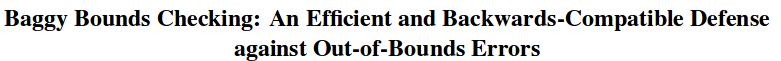
\includegraphics[width=\textwidth]{../bounds/baggy-bounds-title}
\end{frame}

\begin{frame}[fragile,label=lookupTable]{baggy bounds checking idea}
    \begin{itemize}
        \item giant lookup table --- one entry for every 16 bytes of memory
        \item table indicates start of object allocated here
        \item check pointer arithmetic:
    \end{itemize}
\begin{lstlisting}
char p = str[i];
/* becomes: */
CHECK(START_OF[str / 16] == START_OF[&str[i] / 16]);
char p = str[i];
\end{lstlisting}
\end{frame}




\subsection{trick for good performance}

\begin{frame}[fragile,label=baggyBoundsTrick]{baggy bounds trick}
\lstset{language=C,style=small}
    \begin{itemize}
        \item table of pointers to starting locations would be huge
        \item add some restrictions:
            \begin{itemize}
            \item all object sizes are powers of two
            \item all object starting addresses are a multiple of their size
            \end{itemize}
        \item then, table contains size info only:
            \begin{itemize}
            \item table contains $i$, size is $2^i$ bytes:
            \end{itemize}
    \end{itemize}
\begin{lstlisting}
char *GetStartOfObject(char *pointer) {
    return pointer & ~(1 << TABLE[pointer / 16] - 1);
    /* pointer bitwise-and 2^(table entry) - 1 */
    /* clear lower (table entry) bits  of pointer */
}
\end{lstlisting}
\end{frame}



\subsection{the lookup table}
\usetikzlibrary{fit,matrix}

\tikzset{
    stackBox/.style={very thick},
    allocBox/.style={dashed,very thick,fill=blue!20},
    onStack/.style={thick},
    frameOne/.style={fill=blue!15},
    frameTwo/.style={fill=red!15},
    markLine/.style={blue!50!black},
    markLineB/.style={red!90!black},
    hiLine/.style={red!90!black},
}
\begin{frame}<1-6>[fragile,label=lkpTble]{allocations and lookup table}
    \begin{tikzpicture}
        \draw[onStack] (0, 0) rectangle (4, -7);
        \draw[allocBox] (0, 0) rectangle (4, -0.4);
        \draw[stackBox] (0, 0) rectangle (4, -0.5);
        \draw[allocBox] (0, -0.5) rectangle (4, -0.8);
        \draw[stackBox] (0, -0.5) rectangle (4, -1.0);
        \draw[allocBox] (0, -1) rectangle (4, -1.9);
        \draw[stackBox] (0, -1) rectangle (4, -2);
        \draw[allocBox] (0, -2) rectangle (4, -2.4);
        \draw[stackBox] (0, -2) rectangle (4, -2.5);
        \draw[allocBox] (0, -2.5) rectangle (4, -2.7);
        \draw[stackBox] (0, -2.5) rectangle (4, -3);
        \draw[stackBox] (0, -3) rectangle (4, -4);
        \draw[allocBox] (0, -4) rectangle (4, -5.2);
        \draw[stackBox] (0, -4) rectangle (4, -6);

        \begin{visibleenv}<1->
            \node[anchor=north west,align=left] at (9, 0) {
                object allocated in \\ \myemph<1>{power-of-two `slots'}
            };
        \end{visibleenv}
        \begin{visibleenv}<2->
            \matrix[tight matrix,
                nodes={text width=1cm,font=\small\tt},anchor=north west,label={north:table}] (tbl) at (7, -1) {
                $2^4$ \\ $2^4$  \\ $2^5$ \\ $2^5$ \\ $2^4$ \\ $2^4$ \\
                $0$ \\ $0$ \\
                $2^6$ \\ $2^6$ \\ $2^6$ \\ $2^6$ \\
            };
            \begin{scope}[thick,dotted,-Latex]
            \draw (4, -.25) -- (tbl-1-1.west);
            \draw (4, -.75) -- (tbl-2-1.west);
            \draw (4, -1.25) -- (tbl-3-1.west);
            \draw (4, -1.75) -- (tbl-4-1.west);
            \draw (4, -2.25) -- (tbl-5-1.west);
            \draw (4, -2.75) -- (tbl-6-1.west);
            \draw (4, -3.25) -- (tbl-7-1.west);
            \draw (4, -3.75) -- (tbl-8-1.west);
            \draw (4, -4.25) -- (tbl-9-1.west);
            \end{scope}
        \end{visibleenv}
        \begin{visibleenv}<3>
            \draw[ultra thick,red] (0, -1) rectangle (4, -2);
            \node[draw,ultra thick,red,inner sep=0mm,fit=(tbl-3-1) (tbl-4-1)] {};
            \draw[ultra thick,blue] (0, -4) rectangle (4, -6);
            \node[draw,ultra thick,blue,inner sep=0mm,fit=(tbl-9-1) (tbl-12-1)] {};
        \end{visibleenv}
        \begin{visibleenv}<3->
            \node[anchor=north west,align=left] at (9, -2) {
                table stores sizes \\
                \myemph{for each 16 bytes}
            };
        \end{visibleenv}
        \begin{visibleenv}<4>
            \draw[ultra thick,red] (0, -3) rectangle (4, -4);
            \node[draw,ultra thick,red,inner sep=0mm,fit=(tbl-7-1) (tbl-8-1)] {};
        \end{visibleenv}
        \begin{visibleenv}<4->
            \node[anchor=north west,align=left] at (9, -3.5) {
                addresses \textbf<4>{multiples of size} \\
                (may \myemph{require padding})
            };
        \end{visibleenv}
        \begin{pgfonlayer}{bg}
        \begin{visibleenv}<5>
            \fill[red!30] (0, -5.2) rectangle (4, -6.);
            \fill[red!30] (0, -2.7) rectangle (4, -3.);
            \fill[red!30] (0, -1.9) rectangle (4, -2.);
            \fill[red!30] (0, -2.4) rectangle (4, -2.5);
            \fill[red!30] (0, -0.8) rectangle (4, -1.);
            \fill[red!30] (0, -0.4) rectangle (4, -0.5);
        \end{visibleenv}
        \end{pgfonlayer}
        \begin{visibleenv}<5->
            \node[anchor=north west,align=left] at (9, -5.5) {
                sizes are \textbf<5>{powers of two} \\
                (may \myemph{require padding})
            };
        \end{visibleenv}
    \end{tikzpicture}
\end{frame}

\begin{frame}[fragile,label=managing]{managing the table}
    \begin{itemize}
        \item not just done \texttt{malloc()/new}
        \item also for stack allocations:
    \end{itemize}
    \begin{lstlisting}[style=small,language=C]
void vulnerable() {
    char buffer[100];
    gets(vulnerable);
}
\end{lstlisting}
    \begin{tikzpicture}[remember picture, overlay]
        \node[anchor=north east] at ([xshift=-.25cm, yshift=-1cm]current page.north east) {
    \begin{lstlisting}[style=small,language=myasm]
vulnerable:
  // make %rsp a multiple
  // of 128 (2^7) 
  andq $0xFFFFFFFFFFFFFF80, %rsp
  // allocate 128 bytes
  subq $0x80, %rsp
  // rax <- rsp / 16
  movq $rsp, %rax
  shrq $4, %rax
  movb $7, TABLE(%rax)
  movb $7, TABLE+1(%rax)
  ...
  movq %rsp, %rdi
  call gets
  ret
\end{lstlisting}
};
    \end{tikzpicture}
\end{frame}

\begin{frame}[fragile,label=sparseLookup]{sparse lookup table}
    \begin{tikzpicture}
        \node[anchor=south] at (3.5, 3) {lookup table};
        \draw[stackBox] (0, 3) rectangle (7, -3);
        \draw[pattern color=red,pattern=north west lines,onStack] (0, -3) rectangle (7, -1.5)
            node[midway,fill=white,align=center] {unallocated memory (segfault) };
        \draw[fill=green,onStack] (0, -1.5) rectangle (7, .2)
            node[midway] { allocated part of table };
        \draw[pattern color=red,pattern=north west lines,onStack] (0, .20) rectangle (7, 1.3)
            node[midway,fill=white,align=center] {unallocated memory (segfault) };
        \draw[fill=green,onStack] (0, 1.3) rectangle (7, 1.6);
        \draw[pattern color=red,pattern=north west lines,onStack] (0, 1.6) rectangle (7, 2.3);
        \draw[fill=green,onStack] (0, 2.3) rectangle (7, 3)
            node[midway] { allocated part of table };
    \end{tikzpicture}
\end{frame}



\subsection{checks using table}
\usetikzlibrary{calc}
\begin{frame}{baggy bounds check: added code}
    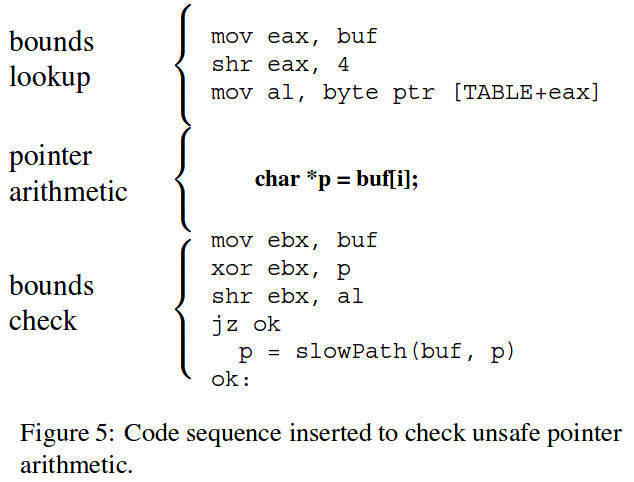
\includegraphics[width=0.6\textwidth]{../bounds/bb-bounds-check}
\end{frame}

\begin{frame}[fragile,label=addedCode]{baggy bounds check: added code}
    \lstset{language=myasm,style=small}
    \begin{lstlisting}
/* bounds lookup */
    mov buf, %rax
    shr %rax, 4
    mov LOOKUP_TABLE(%rax), %al
/* array element address computation */
    ...    // `\textbf{\textit{char * p = buf[i];}}`
/* bound check */
    mov buf, %rbx
    xor p, %rbx
    shr %al, %rbx
    jz  ok
    ...    // handle possible violation
ok:
\end{lstlisting}

    \imagecredit{adapted from paper figure}
\end{frame}

\begin{frame}{avoiding checks}
    \begin{itemize}
        \item code not added if not array/pointer accesses to object
        \item code not added when pointer accesses ``obviously'' safe
            \begin{itemize}
            \item author's implementation: only checked within function
            \end{itemize}
    \end{itemize}
\end{frame}



\subsection{exercise: overhead estimating?}
\begin{frame}<1>[fragile,label=bbOverheadExer1]{exercise: overhead of baggy bounds (1)}
\begin{itemize}
\item suppose program allocates:
    \begin{itemize}
    \item 1000 100 byte objects
    \item 1 10000 byte object
    \end{itemize}
\item using baggy bounds, estimate:
    \begin{itemize}
    \item space required for padding
        \begin{itemize}
        \item<2-> $(128-100)\cdot 1000 + (16384 - 10000)) = 34384$
        \end{itemize}
    \item space required for table
        \begin{itemize}
        \item<2-> $(128\cdot 1000 + 16384) \div 16 = 9024$
        \end{itemize}
    \end{itemize}
\end{itemize}
\end{frame}

\iftoggle{heldback}{}{\againframe<2>{bbOverheadExer1}}

\begin{frame}[fragile,label=bbOverheadExer2]{exercise: overhead of baggy bounds (2)}
\begin{lstlisting}[language=C,style=smaller]
char *strcat(char *d, char *s) {
    int i;
    for (i = 0; s[i] != '\0'; i += 1) {
        d[i] = s[i]; 
    }
    d[i] = '\0';
    return d;
}
\end{lstlisting}
\begin{itemize}
\item estimate:
\begin{itemize}
\item number of bounds checks needed
\item very rough number of instructions run w/o bounds check
\end{itemize}
\item thought question: \\
with bounds checking, what's fastest possible code?
\end{itemize}
\end{frame}


\subsection{alternative: pointer tagging}

\begin{frame}{alternate approach: pointer tagging}
    \begin{itemize}
        \item some bits of \myemph{address} are size 
        \begin{itemize}
        \item replaces table entry/lookup
        \end{itemize}
    \item change code to allocate objects this way
    \item works well on 64-bit --- plenty of addresses to use
    \end{itemize}
    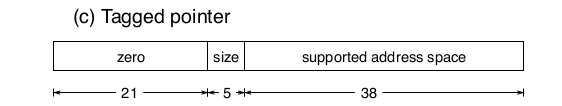
\includegraphics[width=0.8\textwidth]{../bounds/baggy-bounds-tagging}
\end{frame}



\subsection{performance?}

\begin{frame}{baggy bounds performance}
    \begin{itemize}
        \item table: 4--72\% time overhead (depends on benchmark suite)
        \item table: 11--21\% space overhead (depends on benchmark suite)
        \item tagged pointers: slightly better on average
    \end{itemize}
\end{frame}

\begin{frame}{baggy bounds performance}
    \begin{center}
    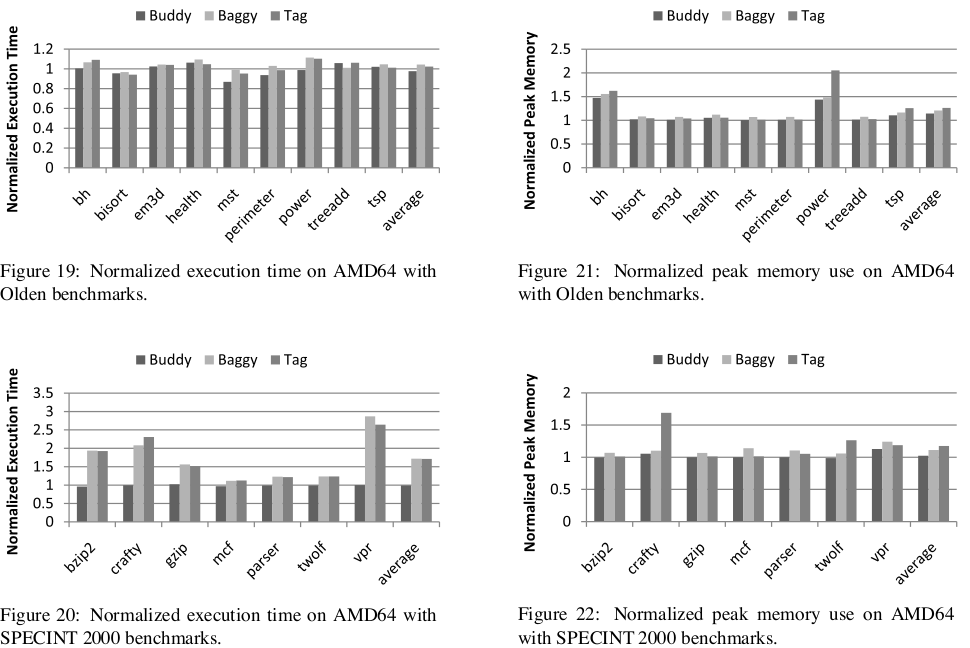
\includegraphics[height=0.8\textheight]{../bounds/baggy-bounds-perf}
    \end{center}
\end{frame}



\subsection{problem: pointers within objects}
% FIXME
\begin{frame}[fragile,label=withinObj]{problem: within object}
\begin{lstlisting}
struct foo {
    char buffer[1024];
    int *pointer;
};
struct foo array_of_foos[1024];
...
char *p = &array_of_foos[4].buffer[4]
\end{lstlisting}
\begin{itemize}
\item exercise: what are the bounds for p?
\end{itemize}
\end{frame}


\subsection{corner cases}

\begin{frame}[fragile,label=unfortunateCProgF2C]{unfortunate things C programmers do (4)}
in code generated by f2c (Fortran to C translator) \\
{\scriptsize (cleaned up slightly)}
\begin{lstlisting}[language=C,style=small]
float sum(int size, float *arr) {
    arr = arr - 1; /* <-- deliberately out-of-bounds pointer */
    float result = 0.f;
    for (i = 1; i <= size; ++i) {
        result += arr[i]
    }
    return result;
}
\end{lstlisting}
\end{frame}



\section{AddressSanitizer}

\begin{frame}{AddressSanitizer}
    \begin{itemize}
    \item like baggy bounds:
        \begin{itemize}
        \item big lookup table
        \item lookup table set by memory allocations
        \item compiler modification: change stack allocations
        \end{itemize}
    \item unlike baggy bounds:
        \begin{itemize}
        \item check reads/writes (instead of pointer computations)
        \item only detect errors that read/write \myemph{between objects}
        \item object sizes not padded to power of two
        \item table has info for every single byte (more precise)
        \end{itemize}
    \end{itemize}
\end{frame}




\subsection{ASan's added check}

\begin{frame}[fragile,label=asanVBounds]{adding bounds-checking example}
\lstset{
    language=C++,
    style=small,
    moredelim={**[is][\btHL<2>]{~2~}{~end~}},
}
\begin{lstlisting}
void vulnerable(long value, int offset) {
    long array[10] = {1,2,3,4,5,6,7,8,9,10};
    // generated code: (added by AddressSanitizer)
    ~2~if (!lookup_table[&array[offset]] == VALID) FAIL();~end~
    array[offset] = value;
    do_something_with(array);
}
\end{lstlisting}
    \begin{itemize}
        \item AddressSanitizer: crashes only if \lstinline|array[offset]| isn't part of any object
            \begin{itemize}
            \item but no extra space --- single-byte precision
            \end{itemize}
    \end{itemize}
\end{frame}



\subsection{stack layout}
\usetikzlibrary{arrows.meta,matrix,patterns}
\tikzset{
    stackBox/.style={very thick},
    allocBox/.style={dashed,very thick,fill=blue!20},
    onStack/.style={thick},
    frameOne/.style={fill=blue!15},
    frameTwo/.style={fill=red!15},
    markLine/.style={blue!50!black},
    markLineB/.style={red!90!black},
    hiLine/.style={red!90!black},
}
\begin{frame}[fragile,label=asanStackLayout]{AddressSanitizer stack layout}
    \begin{tikzpicture}
        \begin{scope}[x=1.7cm]
    \draw[stackBox] (0, 0) rectangle (5, -6);
            \draw[onStack] (0, 0) rectangle (5, -.5)
        node[midway] (arrayLoc) { return address (for \texttt{vulernable()}) };
    \begin{visibleenv}<2>
        \node[anchor=west] at (5.25, -.25) { $\approx$ \tt array[0x13]};
        \node[anchor=west] at (5.25, -3.75) { $\approx$ \tt array[0xa]};
    \end{visibleenv}
    \draw[onStack] (0, -.5) rectangle (5, -1)
        node[midway] { saved \tt\%rbp };
    \draw[onStack] (0, -1) rectangle (5, -1.5)
        node[midway] { saved \tt\%r13 };
    \draw[onStack] (0, -1.5) rectangle (5, -2)
        node[midway] { saved \tt\%r12 };
    \draw[onStack] (0, -2) rectangle (5, -2.5)
        node[midway] { saved \tt\%rbx };
    \draw[onStack,pattern=north west lines,pattern color=red] (0, -2.5) rectangle (5, -4)
        node[midway,fill=white] { ``red zone'' };
    \draw[onStack] (0, -4) rectangle (5, -6)
        node[midway,fill=white] { \tt array };
            \draw[onStack,dashed] (0, -4) rectangle (5, -4.5) node[midway] {\tt array[9]};
            \begin{visibleenv}<3>
            \matrix[tight matrix,
                nodes={text width=3cm,font=\small\tt},anchor=north west,label={north:lookup table}] (tbl) at (6, -2) {
                valid \\ valid  \\ valid \\ valid \\ valid \\ invalid \\ invalid \\
                invalid \\ invalid \\ valid \\ valid \\ \ldots \\
            };
                \draw[thick,-Latex] (5, -.25) -- (tbl-1-1.west);
                \draw[thick,-Latex] (5, -.75) -- (tbl-2-1.west);
            \end{visibleenv}
    \draw[thick,-Latex] (5.15, -6) --++ (0, 2);
        \end{scope}
    \end{tikzpicture}
\end{frame}





\section{AddressSanitizer}

\begin{frame}{AddressSanitizer}
    \begin{itemize}
    \item like baggy bounds:
        \begin{itemize}
        \item big lookup table
        \item lookup table set by memory allocations
        \item compiler modification: change stack allocations
        \end{itemize}
    \item unlike baggy bounds:
        \begin{itemize}
        \item check reads/writes (instead of pointer computations)
        \item only detect errors that read/write \myemph{between objects}
        \item object sizes not padded to power of two
        \item table has info for every single byte (more precise)
        \end{itemize}
    \end{itemize}
\end{frame}




\subsection{ASan's added check}

\begin{frame}[fragile,label=asanVBounds]{adding bounds-checking example}
\lstset{
    language=C++,
    style=small,
    moredelim={**[is][\btHL<2>]{~2~}{~end~}},
}
\begin{lstlisting}
void vulnerable(long value, int offset) {
    long array[10] = {1,2,3,4,5,6,7,8,9,10};
    // generated code: (added by AddressSanitizer)
    ~2~if (!lookup_table[&array[offset]] == VALID) FAIL();~end~
    array[offset] = value;
    do_something_with(array);
}
\end{lstlisting}
    \begin{itemize}
        \item AddressSanitizer: crashes only if \lstinline|array[offset]| isn't part of any object
            \begin{itemize}
            \item but no extra space --- single-byte precision
            \end{itemize}
    \end{itemize}
\end{frame}



\subsection{stack layout}
\usetikzlibrary{arrows.meta,matrix,patterns}
\tikzset{
    stackBox/.style={very thick},
    allocBox/.style={dashed,very thick,fill=blue!20},
    onStack/.style={thick},
    frameOne/.style={fill=blue!15},
    frameTwo/.style={fill=red!15},
    markLine/.style={blue!50!black},
    markLineB/.style={red!90!black},
    hiLine/.style={red!90!black},
}
\begin{frame}[fragile,label=asanStackLayout]{AddressSanitizer stack layout}
    \begin{tikzpicture}
        \begin{scope}[x=1.7cm]
    \draw[stackBox] (0, 0) rectangle (5, -6);
            \draw[onStack] (0, 0) rectangle (5, -.5)
        node[midway] (arrayLoc) { return address (for \texttt{vulernable()}) };
    \begin{visibleenv}<2>
        \node[anchor=west] at (5.25, -.25) { $\approx$ \tt array[0x13]};
        \node[anchor=west] at (5.25, -3.75) { $\approx$ \tt array[0xa]};
    \end{visibleenv}
    \draw[onStack] (0, -.5) rectangle (5, -1)
        node[midway] { saved \tt\%rbp };
    \draw[onStack] (0, -1) rectangle (5, -1.5)
        node[midway] { saved \tt\%r13 };
    \draw[onStack] (0, -1.5) rectangle (5, -2)
        node[midway] { saved \tt\%r12 };
    \draw[onStack] (0, -2) rectangle (5, -2.5)
        node[midway] { saved \tt\%rbx };
    \draw[onStack,pattern=north west lines,pattern color=red] (0, -2.5) rectangle (5, -4)
        node[midway,fill=white] { ``red zone'' };
    \draw[onStack] (0, -4) rectangle (5, -6)
        node[midway,fill=white] { \tt array };
            \draw[onStack,dashed] (0, -4) rectangle (5, -4.5) node[midway] {\tt array[9]};
            \begin{visibleenv}<3>
            \matrix[tight matrix,
                nodes={text width=3cm,font=\small\tt},anchor=north west,label={north:lookup table}] (tbl) at (6, -2) {
                valid \\ valid  \\ valid \\ valid \\ valid \\ invalid \\ invalid \\
                invalid \\ invalid \\ valid \\ valid \\ \ldots \\
            };
                \draw[thick,-Latex] (5, -.25) -- (tbl-1-1.west);
                \draw[thick,-Latex] (5, -.75) -- (tbl-2-1.west);
            \end{visibleenv}
    \draw[thick,-Latex] (5.15, -6) --++ (0, 2);
        \end{scope}
    \end{tikzpicture}
\end{frame}



\subsection{can't change object layout?}
\begin{frame}[fragile,label=withinObj]{revisted: within object}
\begin{lstlisting}
struct foo {
    char buffer[1024];
    int *pointer;
};
struct foo array_of_foos[1024];
...
char *p = &array_of_foos[4].buffer[4]
\end{lstlisting}
\begin{itemize}
\item exercise: What out-of-bounds accesses to `p' can AddressSanitizer detect?
\item how does that compare to baggy bounds? To the `fat pointers' strategy?
\end{itemize}
\end{frame}

\usetikzlibrary{arrows.meta,patterns,shapes.misc}
\tikzset{
    stackBox/.style={very thick},
    allocBox/.style={dashed,very thick,fill=blue!20},
    on stack/.style={thick},
    frameOne/.style={fill=blue!15},
    frameTwo/.style={fill=red!15},
    markLine/.style={blue!50!black},
    markLineB/.style={red!90!black},
    hiLine/.style={red!90!black},
}

\begin{frame}[fragile,label=changeObjLayout]{changing object layout?}
\begin{lstlisting}
struct string_list {
    char data[100];
    struct string_list *prev;
    struct string_list *next;
};
\end{lstlisting}
\begin{tikzpicture}[overlay,remember picture]
\node[anchor=south] at (2.5, 0) {actual layout};
\begin{scope}[shift={(0,0)}]
\draw[on stack] (0, 0) rectangle ++(5, -.5)
    node[midway] {prev};
\draw[on stack] (0, -.5) rectangle ++(5, -.5)
    node[midway] {next};
\draw[on stack] (0, -1) rectangle ++(5, -2)
    node[midway] {data};
\draw[thick,-Latex] (5.25, -3) --++ (0, 1);
\end{scope}
\node[anchor=south] at (9.5, 0) {layout wanted for error-finding};
\begin{scope}[shift={(7,0)}]
\draw[on stack] (0, 0) rectangle ++(5, -.5)
    node[midway] {prev};
\draw[on stack] (0, -.5) rectangle ++(5, -.5)
    node[midway] {next};
\draw[on stack,pattern=north west lines, pattern color=red] (0, -1) rectangle ++(5, -1)
    node[midway] {``red zone''};
\draw[on stack] (0, -2) rectangle ++(5, -2)
    node[midway] {data};
\draw[thick,-Latex] (5.25, -4) --++ (0, 1);
\end{scope}
\begin{visibleenv}<2->
\node[ultra thick,draw,red,cross out,minimum width=5cm,minimum height=4cm] at (9.5, -2) {};
\node[rotate=15,draw,thick,fill=red!10,font=\small,align=center] at (9.5, -3) {
    would break calls to libraries \\
    (unless library also rebuilt)
};
\end{visibleenv}
\end{tikzpicture}
\end{frame}


\subsection{pro/con}

\begin{frame}{AddressSanitizer versus Baggy Bounds}
    \begin{itemize}
    \item pros vs baggy bounds:
        \begin{itemize}
        \item you can actually use it (comes with GCC/Clang)
        \item byte-level precision --- no ``padding'' on objects
        \item detects use-after-free a lot of the time
        \end{itemize}
    \item cons vs baggy bounds:
        \begin{itemize}
        \item doesn't prevent out-of-bounds ``targetted'' accesses
        \item requires extra space between objects
        \item usually slower
        \end{itemize}
    \end{itemize}
\end{frame}



\section{valgrind memcheck, briefly}


\begin{frame}{Valgrind Memcheck}
    \begin{itemize}
    \item similar to AddressSanitizer --- but no compiler modificaitons
    \item instead: is a virtual machine (plus alternate malloc/new implementation)
    \vspace{.5cm}
    \item only (reliably) detects errors on heap
    \item but works on \myemph{unmodified} binaries
    \end{itemize}
\end{frame}




\subsection{aside: binary translation}
% From 20170123
\usetikzlibrary{positioning}

\begin{frame}{binary translation}
    \begin{itemize}
    \item compile assembly to new assembly
    \vspace{1cm}
    \item works without instruction set support
    \item early versions of VMWare on x86 (before x86 added virtualisation support)
    \item can be used to run one platform on another
    \end{itemize}
\end{frame}

\begin{frame}[fragile,label=binTransIdea]{binary translation idea}
\lstset{
    language=myasm,
    style=small,
    morekeywords={movq,addss,subss}
}
\begin{tikzpicture}
\tikzset{
    code/.style={inner sep=0mm,align=left},
    hiOn/.style={alt=#1{rounded corners,fill=green,fill opacity=0.3,text opacity=1.0}{}},
    markOn/.style={alt=#1{rounded corners,draw,thick}{}},
}
\node[code,markOn=<2>,hiOn=<3>] (bb1) {
\begin{lstlisting}
0x40FE00: addq %rax, %rbx
movq 14(%r14,4), %rdx
addss %xmm0, (%rdx)
...
0x40FE3A: jne 0x40F404
\end{lstlisting}
};
\node[right=.25cm of bb1,visible on=<2>,align=left] {
    divide machine code \\
    into \textit{basic blocks} \\
    (= ``straight-line'' code) \\
    (= code till \\ 
    jump/call/etc.)
};
\node[code,right=.25cm of bb1,visible on=<3>] (bb1New) {
generated code: \\
\begin{lstlisting}
// addq %rax, %rbx
movq rax_location, %rdi
movq rbx_location, %rsi
call checked_addq
movq %rax, rax_location
...
// jne 0x40F404
... // get CCs 
je do_jne
movq $0x40FE3F, %rdi
jmp translate_and_run
do_jne:
movq $0x40F404, %rdi
jmp translate_and_run
\end{lstlisting}
};
\node[code,markOn=<2>,anchor=north west] (bb2) at (bb1.south west){
\begin{lstlisting}
subss %xmm0, 4(%rdx)
...
je 0x40F543
\end{lstlisting}
};
\node[code,markOn=<2>,anchor=north west] (bb3) at (bb2.south west){
\begin{lstlisting}
ret
\end{lstlisting}
};
\end{tikzpicture}
\end{frame}

\begin{frame}[fragile,label=binTransIdea2]{a binary translation idea}
    \begin{itemize}
    \item convert whole \textit{basic blocks}
        \begin{itemize}
        \item code upto branch/jump/call
        \end{itemize}
    \item end with call to {\tt translate\_and\_run}
        \begin{itemize}
        \item compute new \myemph{simulated PC} address to pass to call
        \end{itemize}
    \end{itemize}
\end{frame}

\begin{frame}[fragile,label=binTransIdea3]{making binary translation fast}
    \lstset{style=small,language=myasm,morekeywords={movq}}
    \begin{itemize}
    \item cache converted code
        \begin{itemize}
        \item {\tt translate\_and\_run} checks cache first
        \end{itemize}
    \item patch calls to {\tt translate\_and\_run} to refer directly to cached code
    \item do something more clever than \lstinline|movq rax_location, ...|
        \begin{itemize}
        \item map (some) registers to registers, not memory
        \end{itemize}
    \item ends up being ``just-in-time'' compiler
    \end{itemize}
\end{frame}


\begin{frame}{binary translation? really?}
    \begin{itemize}
    \item early VMWare: for instructions without hardware virtualization support
        \begin{itemize}
        \item only needed for little bits of OS code
        \end{itemize}
    \item used by Apple to handle changing CPU designs
    \item Rosetta 2: run Intel on ARM (current)
    \item Rosetta: run Power PC on Intel (2005--2011)
    \item Mac 68k emulator: Run Motorola 680x0 on Power PC (1994--2005)
    \end{itemize}
\end{frame}



\subsection{aside: other binary translation applications}
% FIXME

\section{exericse: which prevents}
\begin{frame}{which scheme prevents\ldots?}
\begin{itemize}
\item which schemes detect or prevent from being harmful\ldots?
    \begin{itemize}
    \item 1. call to assembly code that goes beyond buffer?
    \item 2. allowing attacker to insert 150 bytes in 100 byte buffer on heap?
    \item 3. allowing attacker to insert 120 bytes in 100 byte buffer on stack?
    \item 4. attecker exploiting code that does array[attacker\_index] to overwrite something outside heap array?
    \end{itemize}
\item of:
    \begin{itemize}
    \item A. ``fat pointers'' approach
    \item B. Baggy Bounds checking
    \item C. AddressSanitizer
    \item D. Valgrind Memcheck
    \end{itemize}
\end{itemize}
\end{frame}

\begin{frame}{answer (1)}
\begin{itemize}
\item which schemes detect or prevent from being harmful\ldots?
    \begin{itemize}
    \item 1. call to assembly code that goes beyond buffer?
    \end{itemize}
\item only Valgrind Memcheck handles assembly code
\item other techniques require C compiler to produce different assembly
\end{itemize}
\end{frame}

\begin{frame}{answer (2)}
\begin{itemize}
\item which schemes detect or prevent from being harmful\ldots?
    \begin{itemize}
    \item 2. allowing attacker to insert 150 bytes in 100 byte buffer on heap?
    \end{itemize}
\item schemes:
    \begin{itemize}
    \item A. ``fat pointers'' approach --- yes
    \item B. Baggy Bounds checking ---yes, detect + crash
    \item C. AddressSanitizer --- yes, detect + crash
    \item D. Valgrind Memcheck --- yes, detect + rash
    \end{itemize}
\end{itemize}
\end{frame}

\begin{frame}{answer (3)}
\begin{itemize}
\item which schemes detect or prevent from being harmful\ldots?
    \begin{itemize}
    \item 3. allowing attacker to insert 120 bytes in 100 byte buffer on stack?
    \end{itemize}
\item schemes:
    \begin{itemize}
    \item A. ``fat pointers'' approach --- yes
    \item B. Baggy Bounds checking ---prevent from being harmful / no crash
    \item C. AddressSanitizer --- yes, detect + crash (red zone)
    \item D. Valgrind Memcheck --- no --- no memory to mark invalid
    \end{itemize}
\end{itemize}
\end{frame}

\begin{frame}{answer (3)}
\begin{itemize}
\item which schemes detect or prevent from being harmful\ldots?
    \begin{itemize}
    \item 4. attecker exploiting code that does array[attacker\_index] to overwrite something outside heap array?
    \end{itemize}
\item schemes:
    \begin{itemize}
    \item A. ``fat pointers'' approach --- yes
    \item B. Baggy Bounds checking --- yes
    \item C. AddressSanitizer --- no --- attacher index can find valid memory
    \item D. Valgrind Memcheck --- no --- (same as AddressSanitizer)
    \end{itemize}
\end{itemize}
\end{frame}

% FIXME: exercise
    % which scheme will prevent XXX


\section{backup slides}
\begin{frame}{backup slides}
\end{frame}

\end{document}
